\chapter{Marco Práctico}

El presente capítulo describe la implementación y validación del
simulador neuromórfico desarrollado. Primero se presentan la
arquitectura general del sistema y las herramientas empleadas;
después, la metodología seguida, desde el modelado del dispositivo
memristivo hasta su integración en un agente de control autónomo.
Finalmente, se exponen los resultados de las simulaciones y se
estima el costo de reproducirlas.

Las Etapas 1--4 del desarrollo del sustrato (modelo memristivo y
variabilidad, neurona LIF, plasticidad sináptica y crossbar) se
documentan en ese orden en el Apéndice~\ref{ap:desarrollo_extendido}.
Este capítulo resume su integración en el agente y presenta las
aplicaciones evaluadas, sin asignarles números de etapa adicionales.

% =====================================================
\section{Esquema general del proyecto}
% =====================================================

La solución desarrollada se estructuró como un ecosistema 
computacional compuesto por dos subsistemas acoplados. El 
primero, denominado \textit{Neuromorphic Lab}, constituye el
motor de simulación encargado de modelar dispositivos memristivos,
neuronas tipo Leaky Integrate-and-Fire y arreglos crossbar con 
efectos no ideales. El segundo, denominado \textit{Robot Sim}, 
implementa un agente de control autónomo que utiliza el arreglo 
crossbar simulado como sustrato de pesos de su política.

La Figura~\ref{fig:esquema_general} presenta la organización 
general de ambos subsistemas y su relación unidireccional: el 
simulador robótico consume los modelos físicos del laboratorio 
a través de una capa de abstracción (\textit{lab\_bridge}), 
pero el laboratorio no conoce la existencia del agente.

\begin{figure}[H]
\centering
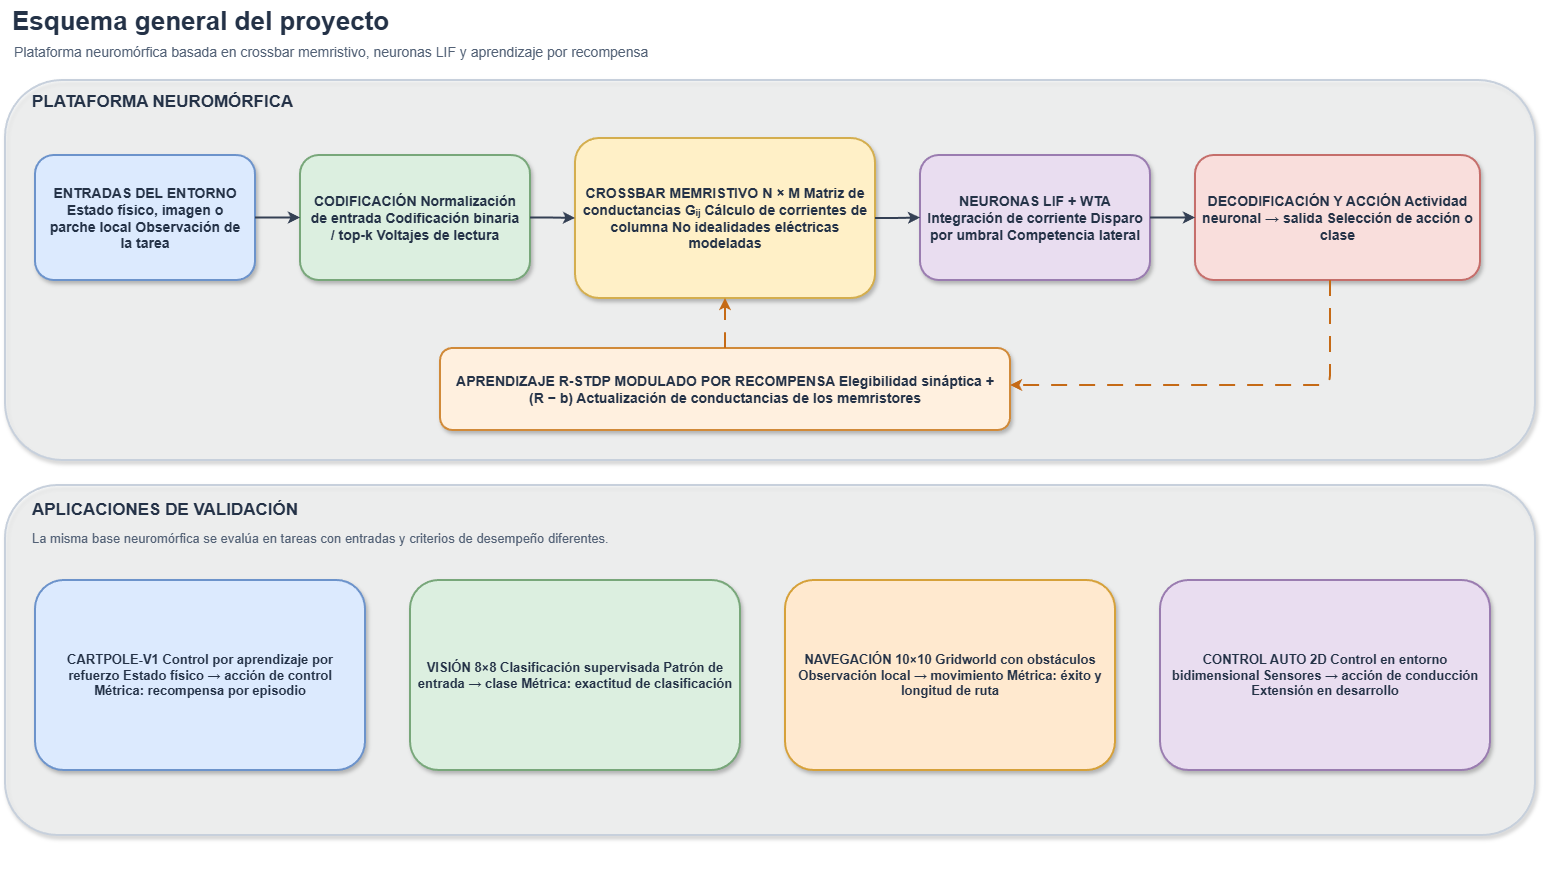
\includegraphics[width=0.86\textwidth]{figuras/esquema_general.png}
\caption[Arquitectura general del ecosistema]{Arquitectura general del ecosistema. El laboratorio 
(\textit{arriba}) provee los modelos físicos; el simulador 
robótico (\textit{abajo}) los integra en un agente de control.}
\label{fig:esquema_general}
\end{figure}

El flujo de información del agente sigue la secuencia 
\textit{sensores} $\rightarrow$ \textit{codificador} 
$\rightarrow$ \textit{crossbar} $\rightarrow$ \textit{decodificador} 
$\rightarrow$ \textit{actuadores}, con el aprendizaje aplicado al 
final de cada episodio mediante una regla de plasticidad 
modulada por recompensa. El detalle de cada componente se 
desarrolla en la Sección~\ref{sec:desarrollo}.

% =====================================================
\section{Herramientas}

El proyecto se desarrolló con herramientas de código abierto,
sin dependencias de software propietario. La Tabla~\ref{tab:hardware} y la
Tabla~\ref{tab:software} listan los componentes principales utilizados.

\subsection{Hardware}

\begin{table}[H]
\centering
\caption{Herramientas de hardware utilizadas.}
\label{tab:hardware}
\begin{tabular}{lp{9cm}}
\hline
\textbf{Componente} & \textbf{Uso} \\
\hline
Laptop de desarrollo & Ejecución de simulaciones y scripts Python (CPU x86-64, 8 GB RAM, SSD) \\
\hline
\end{tabular}
\end{table}

\subsection{Software}

\begin{table}[H]
\centering
\caption{Herramientas de software utilizadas.}
\label{tab:software}
\begin{tabular}{lp{9cm}}
\hline
\textbf{Herramienta} & \textbf{Uso} \\
\hline
Python 3.10+ & Lenguaje principal del simulador \\
NumPy & Álgebra lineal y matrices del crossbar \\
Matplotlib & Generación de figuras y visualización \\
PySide6 & Interfaces gráficas del laboratorio neuromórfico \\
Tkinter & Diálogos de configuración de las aplicaciones \\
Git & Control de versiones \\
\hline
\end{tabular}
\end{table}

% =====================================================

% =====================================================
\section{Metodolog\'ia del agente neurom\'orfico}
\label{sec:metodologia_agente}
\label{sec:desarrollo}

El agente recibe el estado del entorno, lo codifica en entradas del crossbar,
lee sus corrientes de columna y convierte la salida neuronal en una acci\'on.
El arreglo constituye el sustrato de pesos; el entorno y la recompensa se
simulan en software. El desarrollo detallado de los dispositivos, la LIF,
la plasticidad y el solver se documenta en el Ap\'endice~\ref{ap:desarrollo_extendido}.

\subsection{Configuraci\'on de referencia}

CartPole usa un crossbar de $24\times12$, lectura a $0.05\,\mathrm{V}$ y
una neurona LIF por salida. El estado normalizado $X$ se convierte en
resistencia mediante $R(X)=R_{\mathrm{on}}+X(R_{\mathrm{off}}-R_{\mathrm{on}})$;
por ello, $X$ es un estado interno del modelo y no una conductancia. La
configuraci\'on nominal es $R_{\mathrm{on}}=100\,\Omega$,
$R_{\mathrm{off}}=16\,\mathrm{k}\Omega$, $X_0=0.1$ y l\'imites
$0\leq X\leq1$. La tabla resume los par\'ametros el\'ectricos y temporales
usados como referencia.

\begin{table}[H]
\centering
\small
\caption{Par\'ametros de referencia del agente CartPole.}
\label{tab:parametros_agente}
\begin{tabular}{lll}
\toprule
Par\'ametro & Configuraci\'on & Valor efectivo\\
\midrule
$R_{\mathrm{on}}$ & $100\,\Omega$ & $100\,\Omega$\\
$R_{\mathrm{off}}$ & $16\,\mathrm{k}\Omega$ & $16\,000\,\Omega$\\
Estado inicial & $X_0=0.1$ & $x_0=0.9$ bajo $X=1-x$\\
$V_{\mathrm{read}}$ & $0.05\,\mathrm{V}$ & $0.05\,\mathrm{V}$\\
$V_{\mathrm{th}}$ LIF & $1.0\,\mathrm{V}$ & $1.0\,\mathrm{V}$\\
$t_{\mathrm{ref}}$ & $2\,\mathrm{ms}$ & $2\times10^{-3}\,\mathrm{s}$\\
$dt$ & -- & $10^{-4}\,\mathrm{s}$\\
\bottomrule
\end{tabular}
\end{table}

En CartPole, las observaciones se codifican en filas activas; el solver
nodal MNA calcula las corrientes considerando la conductancia del crossbar
y las resistencias configuradas de l\'inea y sensado. Las neuronas LIF
integran las corrientes, generan spikes al alcanzar el umbral y se reinician
seg\'un el per\'iodo refractario. La decisi\'on de acci\'on se obtiene de la
actividad de salida. Estos pasos describen el simulador, no un circuito
fabricado.

La lectura del agente calcula $G(X)$ y resuelve la red MNA sin integrar la
dinamica no volatil del estado durante ese paso; el metodo de lectura no
llama a la actualizacion de las celdas, por lo que en esta ruta simulada
$\Delta X=0$ por construccion. Esto cuantifica el cambio de estado impuesto
por el software en cada lectura, no una perturbacion electrica medida en un
dispositivo fisico. El modelo Strukov del laboratorio si incorpora un
umbral de deriva ionica de $0.1\,\mathrm{V}$ como valor predeterminado
de \texttt{StrukovConfig}; ese umbral se aplica al integrar la dinamica de la celda y no es una medicion
experimental del umbral del dispositivo. El dispositivo volatil de salida,
en cambio, si se actualiza en cada paso y modula la corriente que recibe
la LIF.

\subsection{Reglas de aprendizaje y decisi\'on}

En REINFORCE, el agente conserva una elegibilidad por conexi\'on durante el
episodio y la actualiza al terminarlo seg\'un el retorno y un baseline. La
contribuci\'on instant\'anea es
\[
e_{ij,t}=\mathrm{pre}_{i,t}
\left(\mathbf{1}_{j=\mathrm{col}_t}-\pi_{j,t}\right),\qquad
E_{ij,t}=\gamma E_{ij,t-1}+e_{ij,t},
\]
donde $\pi_{j,t}$ es la probabilidad softmax de la columna $j$. La softmax
convierte puntuaciones en probabilidades que suman uno: una temperatura alta
reparte m\'as la probabilidad y una baja la concentra. El decoder muestrea
seg\'un esa distribuci\'on y la regla de aprendizaje ajusta el crossbar con el
resultado del episodio. Esta forma de gradiente de pol\'itica se basa en REINFORCE y en los m\'etodos
de aprendizaje por refuerzo descritos en la literatura~\cite{Williams1992REINFORCE,SuttonBarto2018}. La implementaci\'on se describe en
\url{robot_sim/neurobot/reinforce_agent.py} y
\url{robot_sim/neurobot/crossbar_brain.py}.

La regla local STDP del laboratorio usa spikes binarios pre/post y trazas
exponenciales $p_i$ y $q_j$:
\[
\tau_{\mathrm{pre}}\dot p_i=-p_i+s_i^{\mathrm{pre}},\qquad
\tau_{\mathrm{post}}\dot q_j=-q_j+s_j^{\mathrm{post}},\qquad
\Delta G_{ij}^{\mathrm{STDP}}=\eta\left(A_+p_i s_j^{\mathrm{post}}
-A_-s_i^{\mathrm{pre}}q_j\right).
\]
En la regla R-STDP del m\'odulo, la elegibilidad decae y acumula ese cambio:
\[
E_{ij,t}=e^{-dt/\tau_e}E_{ij,t-1}+\Delta G_{ij,t}^{\mathrm{STDP}},
\qquad \Delta G_{ij,t}^{\mathrm{R-STDP}}=R_tE_{ij,t}.
\]
Esta formulaci\'on de elegibilidad modulada por recompensa sigue el marco
conceptual de R-STDP~\cite{Izhikevich2007RSTD}; en este proyecto, la regla
local implementada se describe en \url{neurolab/crossbar/plasticity.py}.

Las corridas del agente etiquetadas R-STDP en el Ap\'endice
\ref{ap:evidencia_entrenamientos} no implementan esa regla estricta con
spikes LIF como evento post. En los entornos de control, el runner construye
un evento de acci\'on centrado por la pol\'itica,
$z_{j,t}=\mathbf{1}_{j=a_t}-\pi_{j,t}$, y una elegibilidad por decisi\'on
$e_{ij,t}=a_+\,\mathrm{pre}_{i,t}\max(z_{j,t},0)
+a_-\,\mathrm{pre}_{i,t}\min(z_{j,t},0)$. Los spikes LIF y los ganadores
WTA se registran, pero no sustituyen a $z_{j,t}$ en esta actualizaci\'on;
la tarea de visi\'on usa una elegibilidad derivada del gradiente de corriente.
Para cada paso se calcula el retorno descontado $G_t=r_t+\gamma G_{t+1}$,
la ventaja $A_t=G_t-b_t$ respecto al baseline temporal previo y su
normalizaci\'on $\widehat A_t=A_t/s_A$, donde
$s_A=\max(\operatorname{std}(A),10^{-8})$ (se usa $s_A=1$ para un solo
paso). La elegibilidad modulada del episodio es
\[
E^R_{ij}=\frac{1}{\sqrt{T}}\sum_{t=0}^{T-1} e_{ij,t}\widehat A_t,
\qquad \Delta X=-\eta E^R.
\]
El cambio se escala para cumplir el l\'imite configurado de
$\max_{ij}|\Delta X_{ij}|$ y se anula en episodios que alcanzan el umbral
de congelamiento. La actualizaci\'on opera directamente sobre el estado
abstracto $X$ y las variabilidades D2D/C2C modifican el incremento aplicado.
Para $E^R>0$, $\Delta X<0$ reduce $R(X)$ y aumenta $G(X)$; el signo opuesto
produce el efecto contrario. Esta comprobaci\'on algebraica confirma la
direcci\'on del mapeo en el c\'odigo, pero no demuestra aprendizaje estable
ni programaci\'on por pulsos f\'isicos. Por ello, en
esta tesis las corridas del runner se describen como el piloto h\'ibrido
pre/acci\'on modulado por retorno (conservando R-STDP como nombre del modo
del software), no como evidencia de R-STDP can\'onica pre/post. La variante
de tarea que s\'i emple\'o spikes LIF reales como evento post tuvo bajo
rendimiento exploratorio. Los resultados y su alcance se informan en la
Secci\'on~\ref{sec:piloto_rstdp_reinforce}; la topolog\'ia y el modelo
el\'ectrico del crossbar se mantienen entre reglas de aprendizaje.

\subsection{Aplicaciones evaluadas}

La misma organizaci\'on se adapt\'o a cuatro tareas. Se conservaron la lectura
del crossbar y la actualizaci\'on por recompensa; las dimensiones y el
significado de la salida dependen del entorno. Los registros por condici\'on
se incluyen en el Ap\'endice~\ref{ap:evidencia_entrenamientos}.

\begin{table}[H]
\centering
\small
\caption{Configuraci\'on de las aplicaciones simuladas.}
\label{tab:aplicaciones}
\begin{tabularx}{\textwidth}{l c X X}
\toprule
Tarea & Crossbar & Entrada y salida & M\'etrica\\
\midrule
CartPole & $24\times12$ & Estado continuo; dos acciones & Recompensa y supervivencia\\
Visi\'on & $64\times8$ & Patr\'on binario $8\times8$; ocho clases & Exactitud\\
Obst\'aculos & $16\times4$ & Sensores del gridworld; cuatro movimientos & Llegada a meta\\
Auto 2D & $24\times8$ & Rayos, direcci\'on y distancia; cuatro controles & Llegada a meta\\
\bottomrule
\end{tabularx}
\end{table}

\section{Validaci\'on de modelos}
\label{sec:validacion_modelos}

La validaci\'on se organiz\'o en tres niveles: comprobaciones internas de
c\'odigo y unidades, comparaci\'on de series simuladas con puntos digitalizados
de publicaciones y pruebas funcionales de las aplicaciones. Solo se
presentan m\'etricas cuando existe correspondencia punto a punto y protocolo
definido. Una coincidencia visual, una distribuci\'on sint\'etica o una traza
producida por el mismo modelo no equivalen a una medici\'on de hardware. El
inventario de fuentes y scripts est\'a en el ap\'endice de datos; los protocolos
completos se conservan en el Ap\'endice~\ref{ap:desarrollo_extendido}.

\begin{figure}[H]
\centering
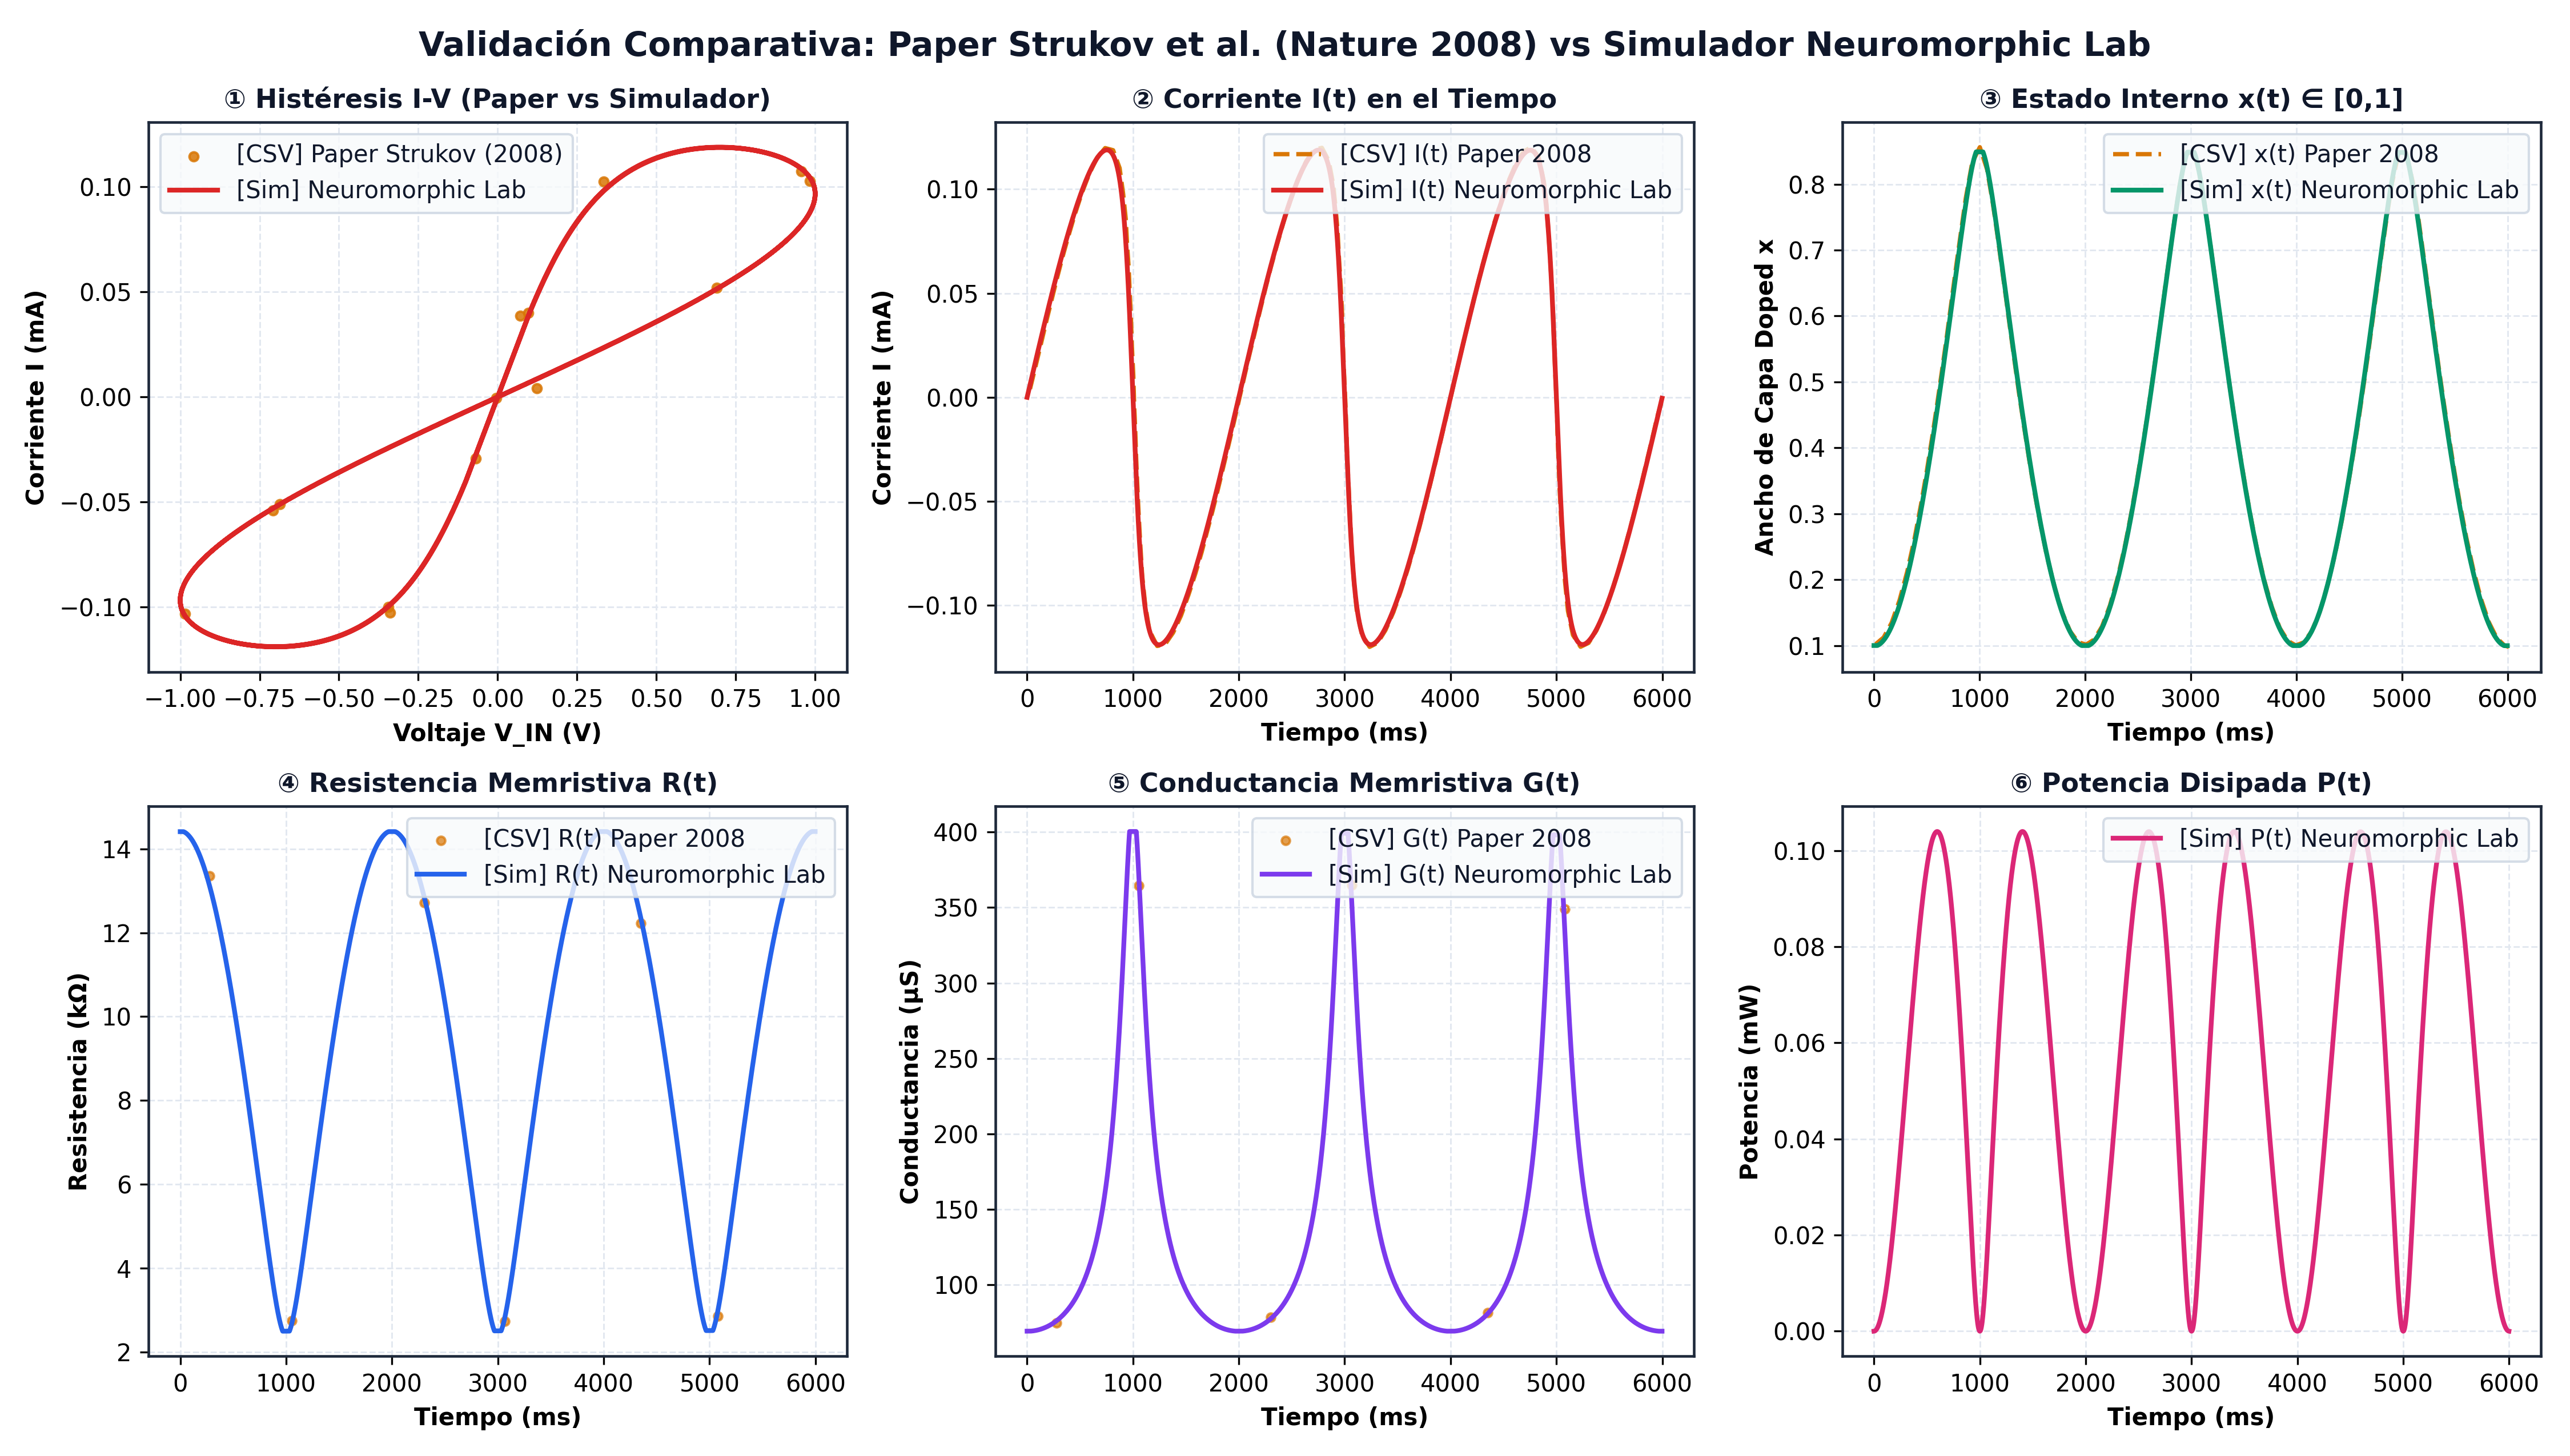
\includegraphics[width=0.78\textwidth]{figuras/fig_01_strukov.png}
\caption{Curvas del modelo Strukov local comparadas con las series digitalizadas atribuidas a la referencia.}
\label{fig:strukov_iv}
\end{figure}

\subsection{Comparaciones cuantitativas}

Para Strukov se compararon estado, corriente, resistencia y conductancia
con series digitalizadas atribuidas al art\'iculo de 2008. Prezioso es una
comparaci\'on visual, pues los puntos no contienen protocolo temporal
completo. La ventana STDP usa nueve puntos de ajuste y cuatro reservados;
LTP/LTD usa 18 puntos de test. La LIF $f-I$ compara Euler con la soluci\'on
anal\'itica del mismo modelo, no con mediciones experimentales. La tabla
resume las m\'etricas reproducibles.

\begin{table}[H]
\centering
\footnotesize
\caption{M\'etricas de validaci\'on reproducibles. $R^2$ es el coeficiente de determinaci\'on; ERP se normaliza por el rango de referencia.}
\label{tab:metricas_validacion}
\begin{tabularx}{\textwidth}{X c c c c c}
\toprule
Comparaci\'on & $n$ & $R^2$ & MAE & RMSE & ERP (\%)\\
\midrule
Strukov, estado $x(t)$ &107&0.999657&0.003676&0.004491&1.27\\
Strukov, corriente $I(t)$ &136&0.996994&0.002586 mA&0.004126 mA&6.22\\
Strukov, resistencia $R(t)$ &87&0.998319&0.135431 k$\Omega$&0.162264 k$\Omega$&3.54\\
Strukov, conductancia $G(t)$ &87&0.983726&7.55759 $\mu$S&15.64415 $\mu$S&19.04\\
Prezioso, $I(V)$ visual &179&--&--&--&--\\
STDP, holdout &4&0.94220&1.90404 pp&2.13626 pp&14.87\\
LTP/LTD, test &18&0.73988&8.3491 nA&8.6181 nA&31.23\\
LIF $f-I$, Euler vs anal\'itica &14&0.999964&0.086431 Hz&0.151393 Hz&0.55\\
\bottomrule
\end{tabularx}
\end{table}

STDP y LTP/LTD proceden de conjuntos digitalizados peque\~nos; sus par\'ametros
ajustados son efectivos y no caracterizan independientemente un dispositivo.
En LTP/LTD, el resultado agregado oculta un ajuste deficiente por rama.
Prezioso carece de etiquetas temporales y de rama suficientes para una
m\'etrica. La prueba D2D/C2C verifica propiedades estad\'isticas de muestras
sint\'eticas, no una poblaci\'on experimental. Las Figuras
\ref{fig:stdp_curve_ch3} y \ref{fig:ltp_ltd_curve_ch3} permiten inspeccionar
los datos atribuidos a Jo et al.; las particiones y limitaciones se ampl\'ian
en el ap\'endice t\'ecnico.

\begin{table}[H]
\centering
\footnotesize
\caption{Cumplimiento de los umbrales cuantitativos cuando son aplicables.}
\label{tab:estado_criterios_modelos}
\begin{tabularx}{\textwidth}{l c c X}
\toprule
Prueba & ERP $<10\%$ & $R^2>0.90$ & Conclusi\'on\\
\midrule
Strukov: $x$, $I$, $R$ & S\'i & S\'i & Cumplen en las series comparadas.\\
Strukov: $G$ & No & S\'i & ERP $=19.04\%$; no cumple todos los umbrales.\\
STDP, holdout ($n=4$) & No & S\'i & Parcial; ERP $=14.87\%$ y muestra peque\~na.\\
LTP/LTD ($n=18$) & No & No & No cumple; $R^2=0.73988$, ERP $=31.23\%$.\\
Prezioso $I(V)$ & No calculable & No calculable & Comparaci\'on visual; faltan puntos con protocolo suficiente.\\
LIF $f-I$ & S\'i$^*$ & S\'i$^*$ & Verificaci\'on interna frente a soluci\'on anal\'itica, no validaci\'on experimental independiente.\\
\bottomrule
\end{tabularx}
\par\smallskip\scriptsize $^*$M\'etricas de integraci\'on para el mismo modelo anal\'itico; no se interpretan como concordancia con hardware publicado.
\end{table}

\begin{figure}[H]
\centering
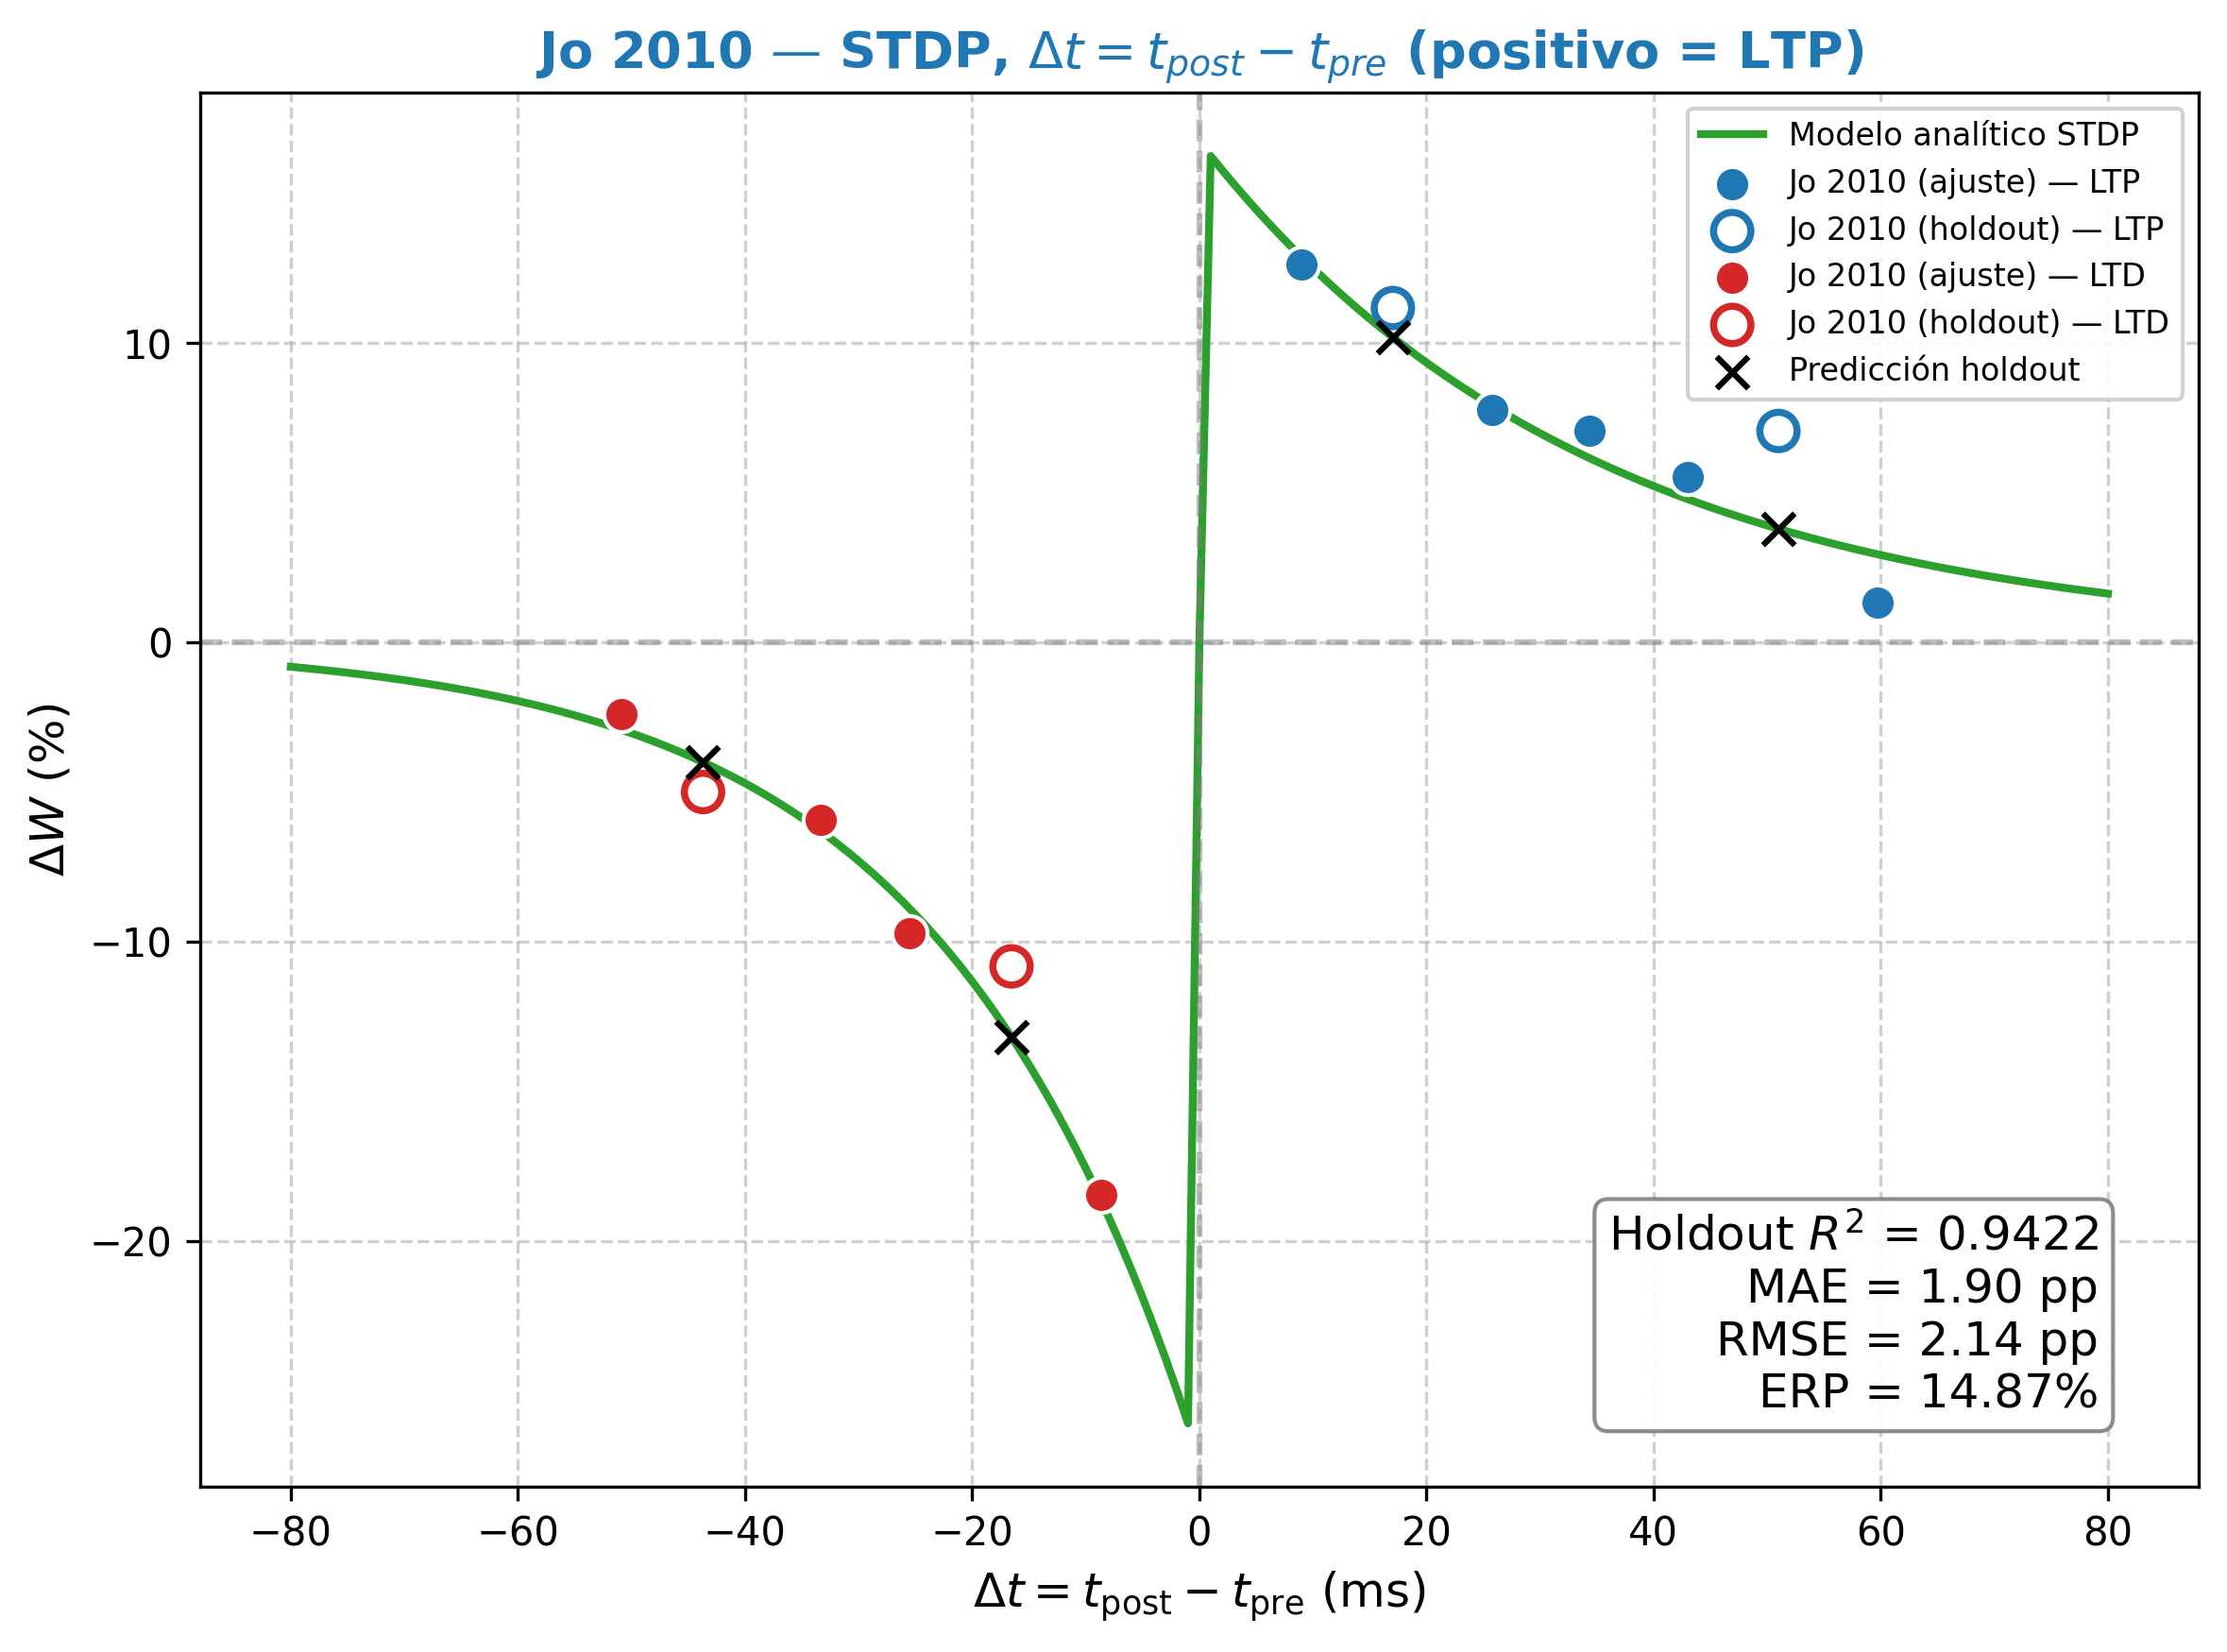
\includegraphics[width=0.72\textwidth]{figuras/fig_15b_stdp_jo2010.png}
\caption{Ajuste STDP en nueve puntos y evaluaci\'on en cuatro puntos reservados atribuidos a Jo et al. (2010).}
\label{fig:stdp_curve_ch3}
\end{figure}
\begin{figure}[H]
\centering
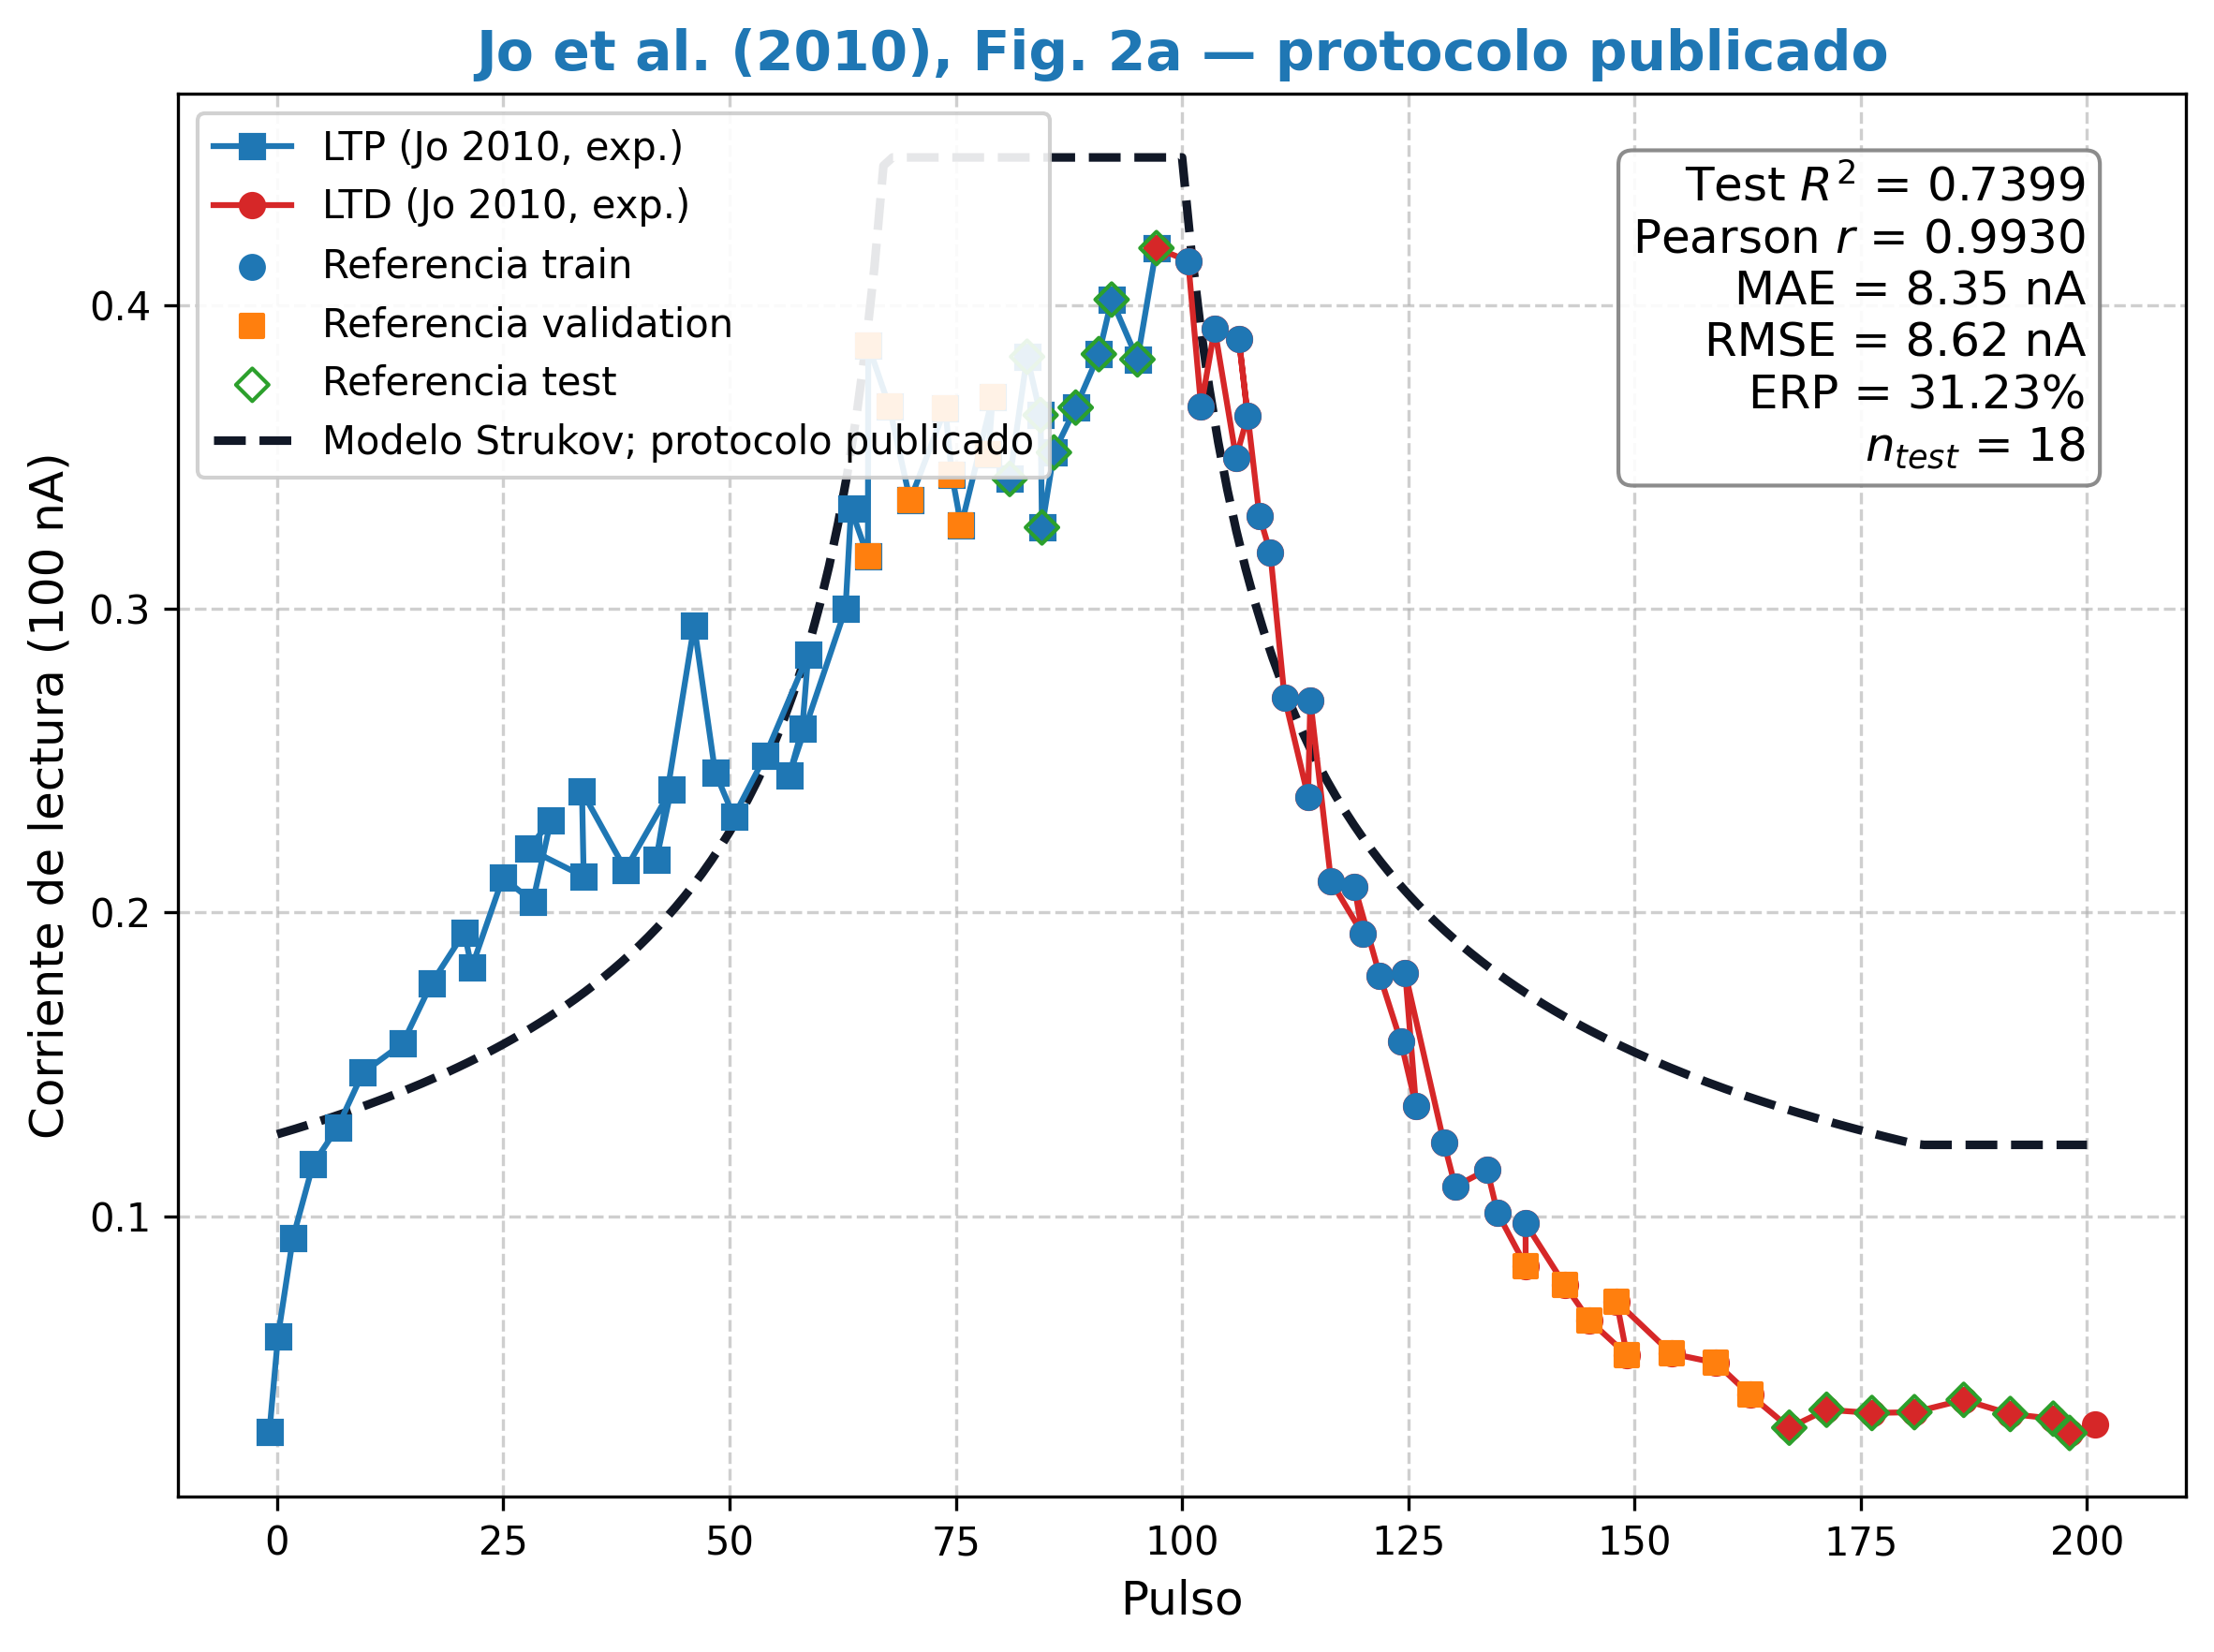
\includegraphics[width=0.72\textwidth]{figuras/fig_14b_ltp_ltd_jo2010.png}
\caption{Comparaci\'on LTP/LTD atribuida a Jo et al. (2010); los par\'ametros se ajustaron con datos de entrenamiento.}
\label{fig:ltp_ltd_curve_ch3}
\end{figure}

\begin{table}[H]
\centering
\small
\caption{Cumplimiento de objetivos seg\'un el alcance de la evidencia.}
\label{tab:cumplimiento_objetivos}
\begin{tabularx}{\textwidth}{l X l}
\toprule
Objetivo & Evidencia resumida & Estado\\
\midrule
Modelos memristivos y variabilidad & Comparaciones digitalizadas y pruebas sint\'eticas; alcance acotado. & Parcial\\
Neurona LIF & Disparo, reinicio, refractario y curva $f-I$ frente a soluci\'on anal\'itica. & Verificado internamente\\
Plasticidad local & STDP con cuatro puntos reservados; conjunto peque\~no. & Parcial\\
Crossbar & Solver MNA y comprobaci\'on num\'erica; sin medici\'on f\'isica. & Verificado en simulaci\'on\\
Aprendizaje de tareas & REINFORCE de referencia y piloto R-STDP con resultados variables. & Parcial\\
\bottomrule
\end{tabularx}
\end{table}

\subsection{Verificaci\'on del sistema integrado}
\label{sec:crossbar_manual}

Se verific\'o la conversi\'on de unidades, un caso manual de crossbar $2\times2$
y la invariancia de pesos durante evaluaciones congeladas. La respuesta LIF
se contrast\'o con la soluci\'on anal\'itica frecuencia--corriente; la prueba
temporal comprueba umbral, reinicio y refractario en el propio modelo. El
Ap\'endice t\'ecnico distingue estas verificaciones de una validaci\'on f\'isica.

La prueba manual usa $G=[[0.001,0.0005],[0.00033333,0.00025]]\,\mathrm{S}$ y
$V=[0.05,0]^{\mathsf T}\,\mathrm{V}$. La multiplicaci\'on ideal produce
$[50,25]~\mu\mathrm{A}$; el solver MNA produce $[44.1176,23.2558]~\mu\mathrm{A}$.
La diferencia corresponde a las resistencias del protocolo del solver, no a
la identidad matricial ideal.

\begin{figure}[H]
\centering
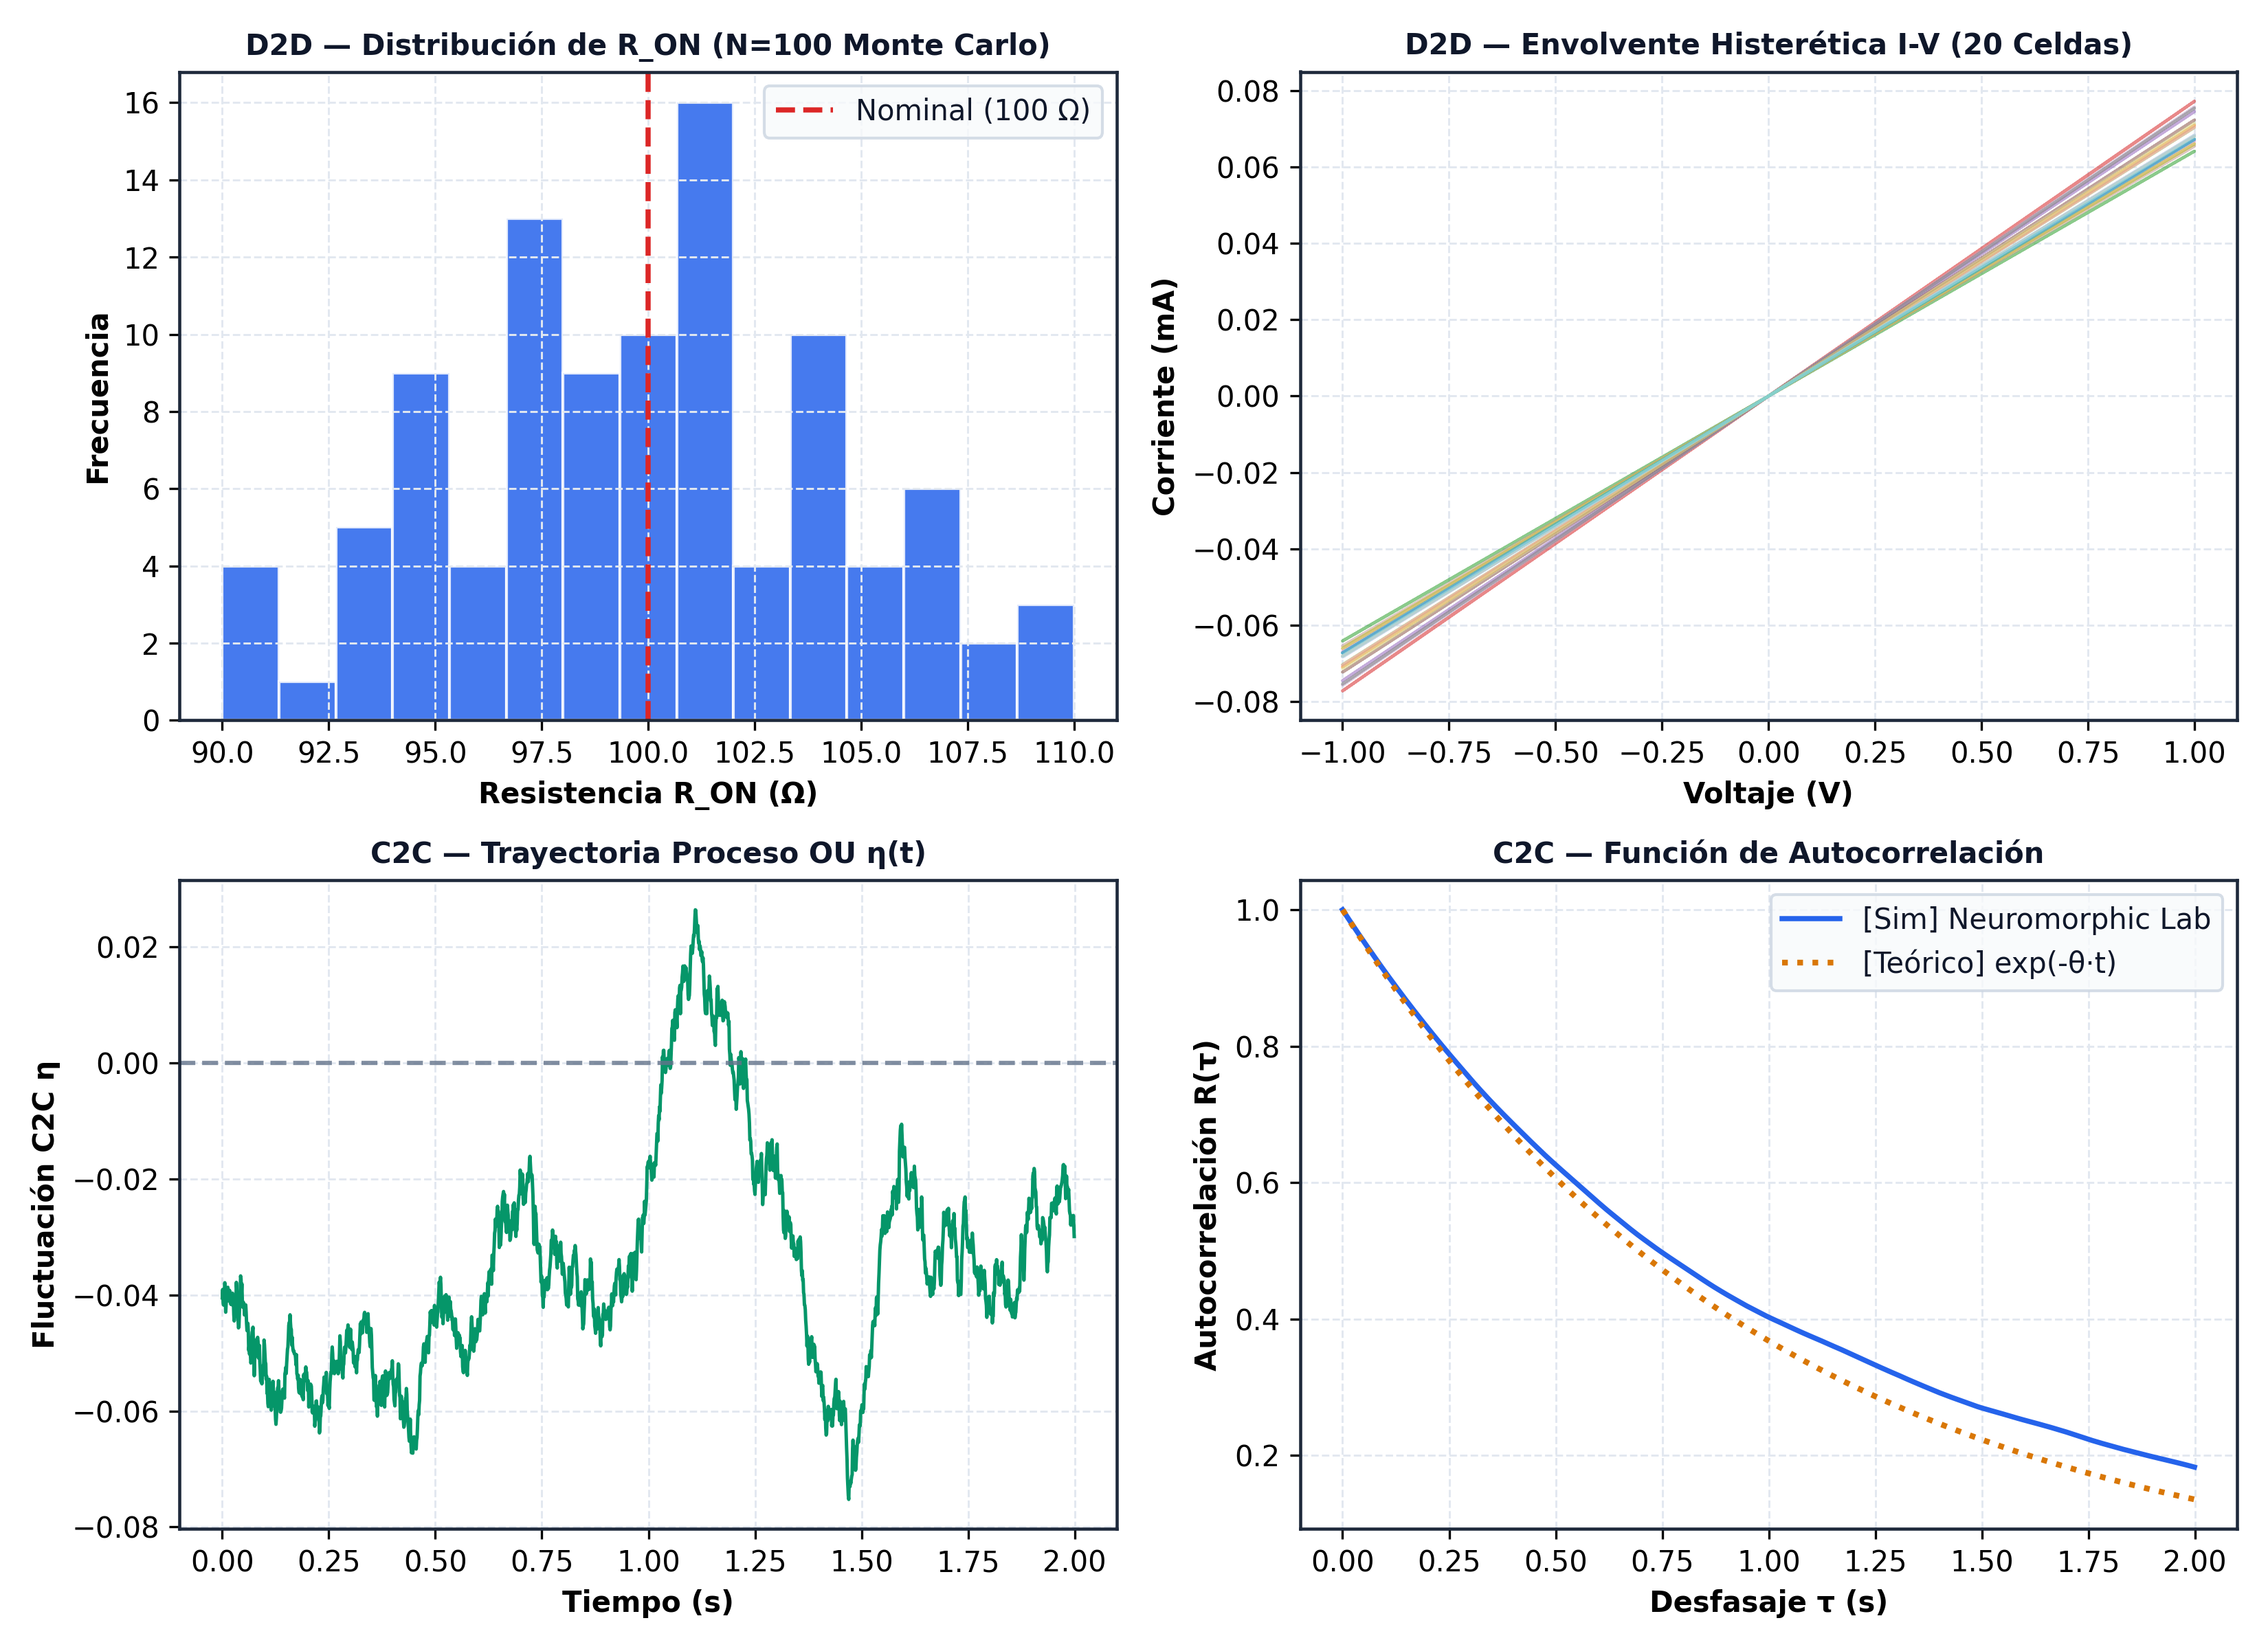
\includegraphics[width=0.67\textwidth]{figuras/fig_05_d2d_c2c.png}
\caption{Distribuciones sint\'eticas D2D/C2C del modelo y sus referencias te\'oricas; no son histogramas de mediciones f\'isicas.}
\label{fig:d2d_c2c_validation}
\end{figure}

\begin{figure}[H]
\centering
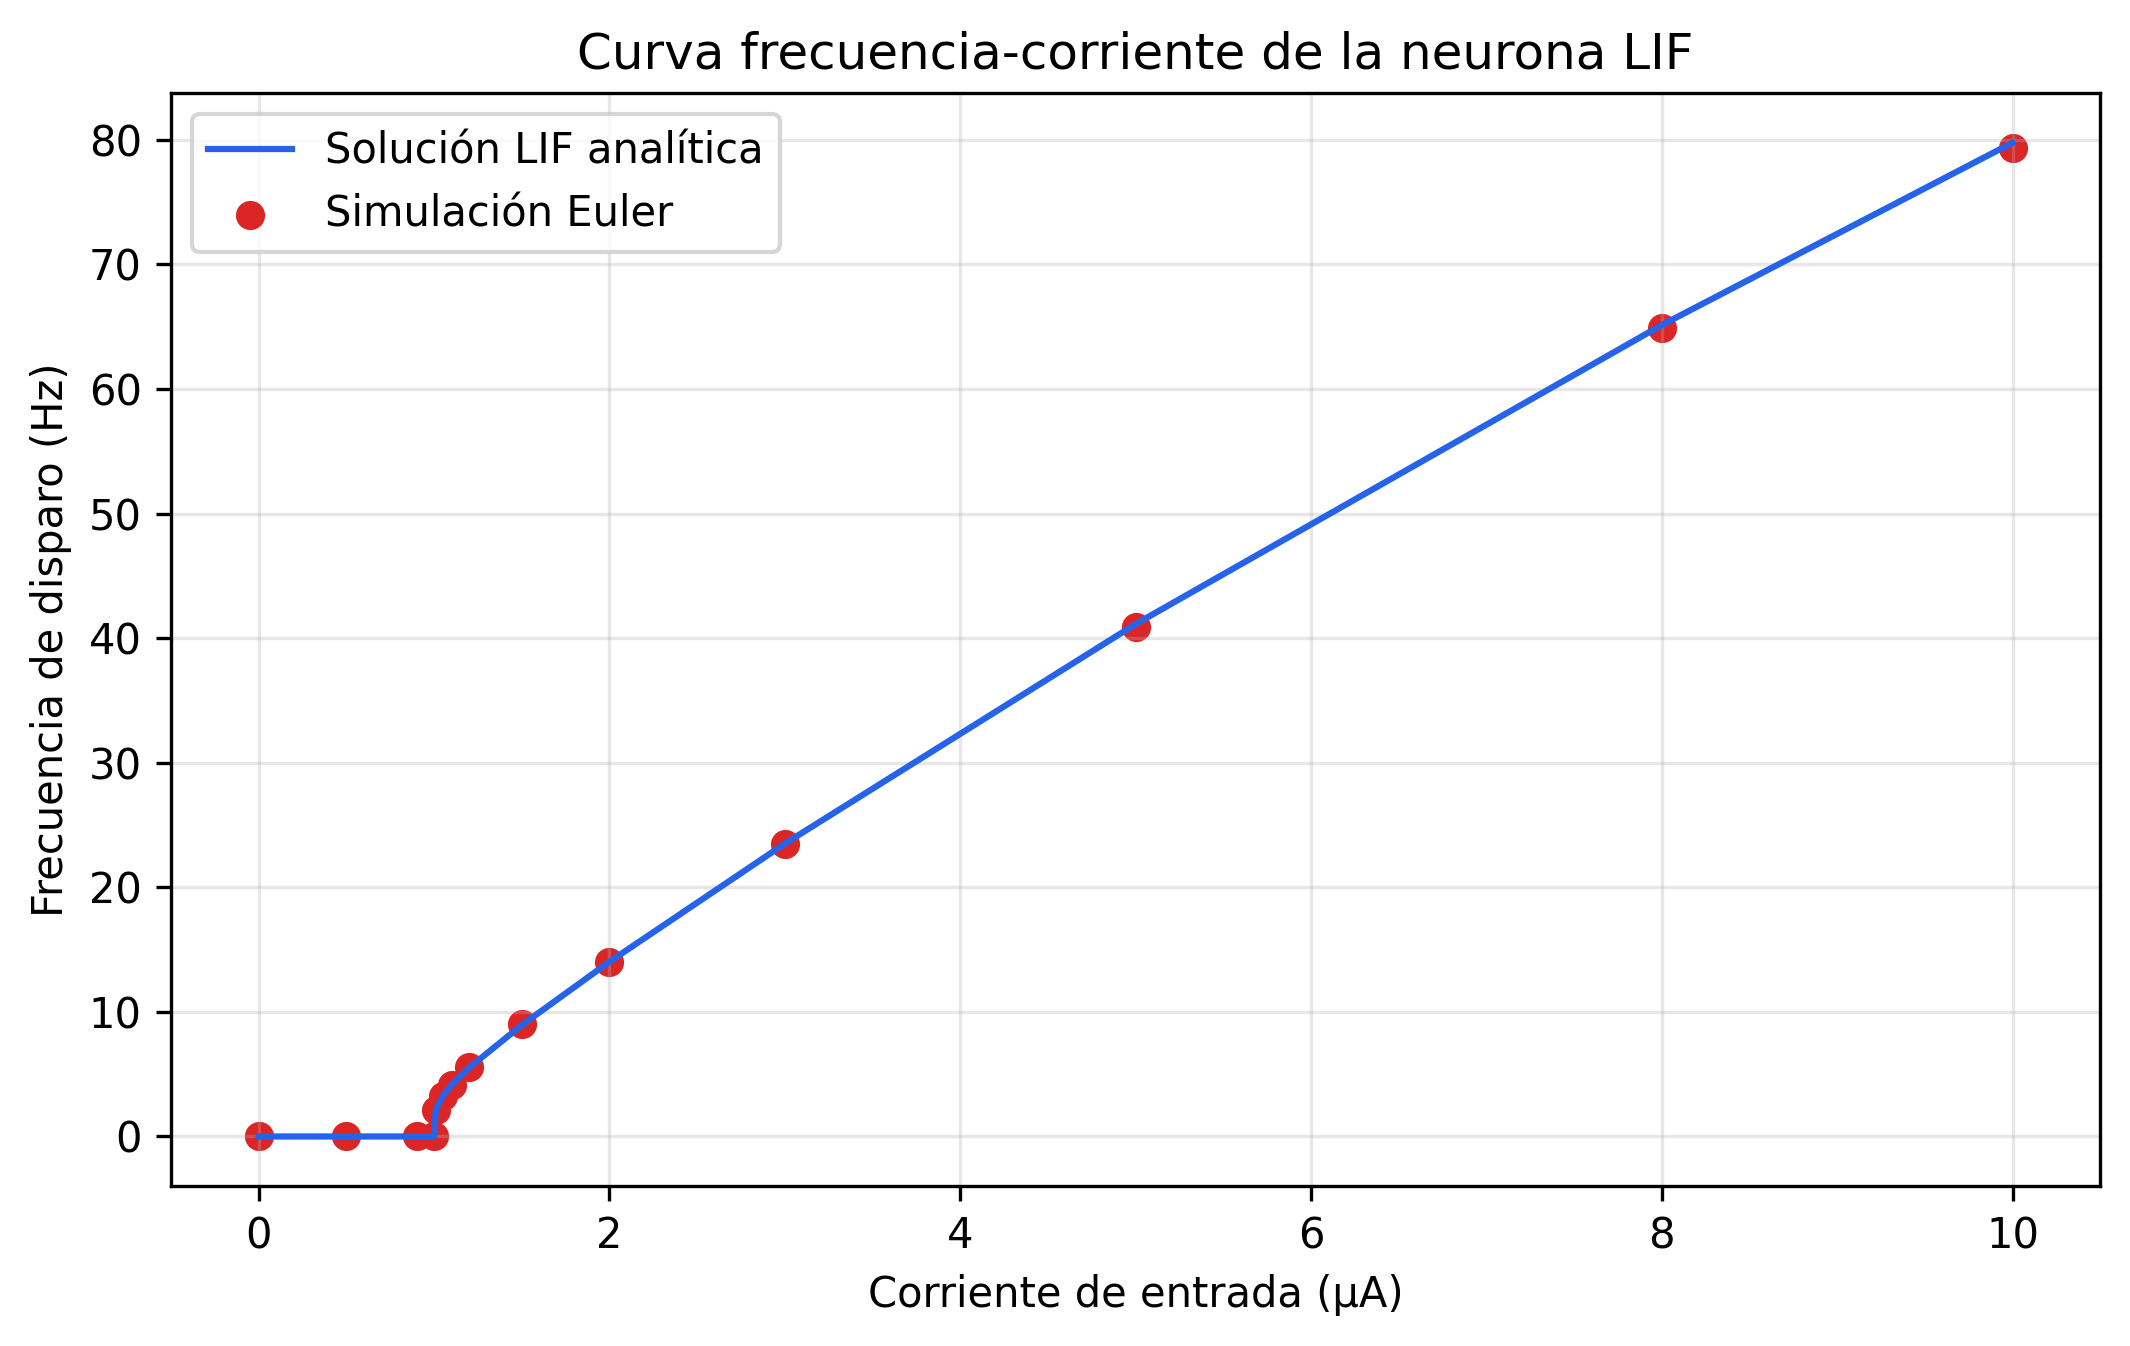
\includegraphics[width=0.67\textwidth]{figuras/lif_fi_curve.png}
\caption{Frecuencia de disparo LIF por Euler frente a la soluci\'on anal\'itica del mismo modelo.}
\label{fig:lif_fi_curve}
\end{figure}

\section{Resultados y discusi\'on}
\label{sec:resultados}

Las m\'etricas de cada aplicaci\'on son espec\'ificas y no se interpretan como
comparaci\'on controlada cuando cambian la arquitectura, la recompensa o el
presupuesto de entrenamiento. Los registros y matrices por condici\'on est\'an
en el Ap\'endice~\ref{ap:evidencia_entrenamientos}.


\begin{table}[H]
\centering
\scriptsize
\setlength{\tabcolsep}{3pt}
\caption{Separaci\'on de entrenamiento, validaci\'on y test en las aplicaciones.}
\label{tab:train_validation_test_tasks}
\begin{tabularx}{\textwidth}{l X X X}
\toprule
Tarea & Entrenamiento & Validaci\'on y selecci\'on & Test independiente\\
\midrule
CartPole & Cinco semillas, 300 episodios cada una. & 50 episodios por checkpoint; se selecciona semilla 4 ($493.77$). & 50 episodios, semillas 20000--20049; $493.63\pm0.93$.\\
Visi\'on & Tres semillas, 5000 episodios sobre ocho plantillas. & 160 variantes por checkpoint con inversi\'on de p\'ixel $p=0.05$; selecci\'on: semilla 2 ($42.5\%$). & 400 variantes nuevas; exactitud $42.5\%$.\\
Obst\'aculos & Semillas 0--2; 746, 800 y 800 episodios. & 20 mapas por checkpoint; selecci\'on: semilla 2 ($25\%$). & 50 mapas nuevos; \'exito $4\%$ (2/50).\\
Auto 2D & Una semilla; horizonte reportado de 3000 episodios y snapshots cada 200. & 20 escenarios por snapshot; checkpoint reportado con $15\%$. & 50 escenarios; \'exito reportado $14\%$ (7/50); faltan logs para recalcular.\\
\bottomrule
\end{tabularx}
\end{table}

\subsection{CartPole-v1: control con recompensa densa}
\label{sec:res_cartpole}

Se entren\'o el agente $24\times12$ durante 300 episodios en cinco semillas,
con D2D/C2C y supresi\'on de actualizaci\'on en cada episodio cuya recompensa
alcanz\'o 430. La recompensa media de los \'ultimos 200 episodios fue 369.66,
421.44, 474.31, 462.79 y 448.36 para las semillas 0--4 (media $435.31$,
desviaci\'on est\'andar $37.28$). Cuatro corridas alcanzaron una recompensa
epis\'odica de 480. El umbral omite una actualizaci\'on de pesos de ese episodio,
pero no congela permanentemente el agente.

Para evaluar dentro de la tarea, se seleccion\'o en validaci\'on el checkpoint
de la semilla 4 y se evalu\'o sin aprendizaje en 50 episodios de test
independientes. Obtuvo $493.63\pm0.93$ puntos (rango 490.43--494.94);
$X$ no cambi\'o y el decoder fue greedy. En la comparaci\'on emparejada
ideal--D2D/C2C, la diferencia media fue $+99.46\pm226.90$ puntos, pero
solo tres de cinco pares favorecieron la condici\'on variable; el resultado
es descriptivo y no prueba una ventaja general. La curva de cinco semillas
est\'a en la Figura~\ref{fig:cartpole_learning}.

\begin{figure}[H]
\centering
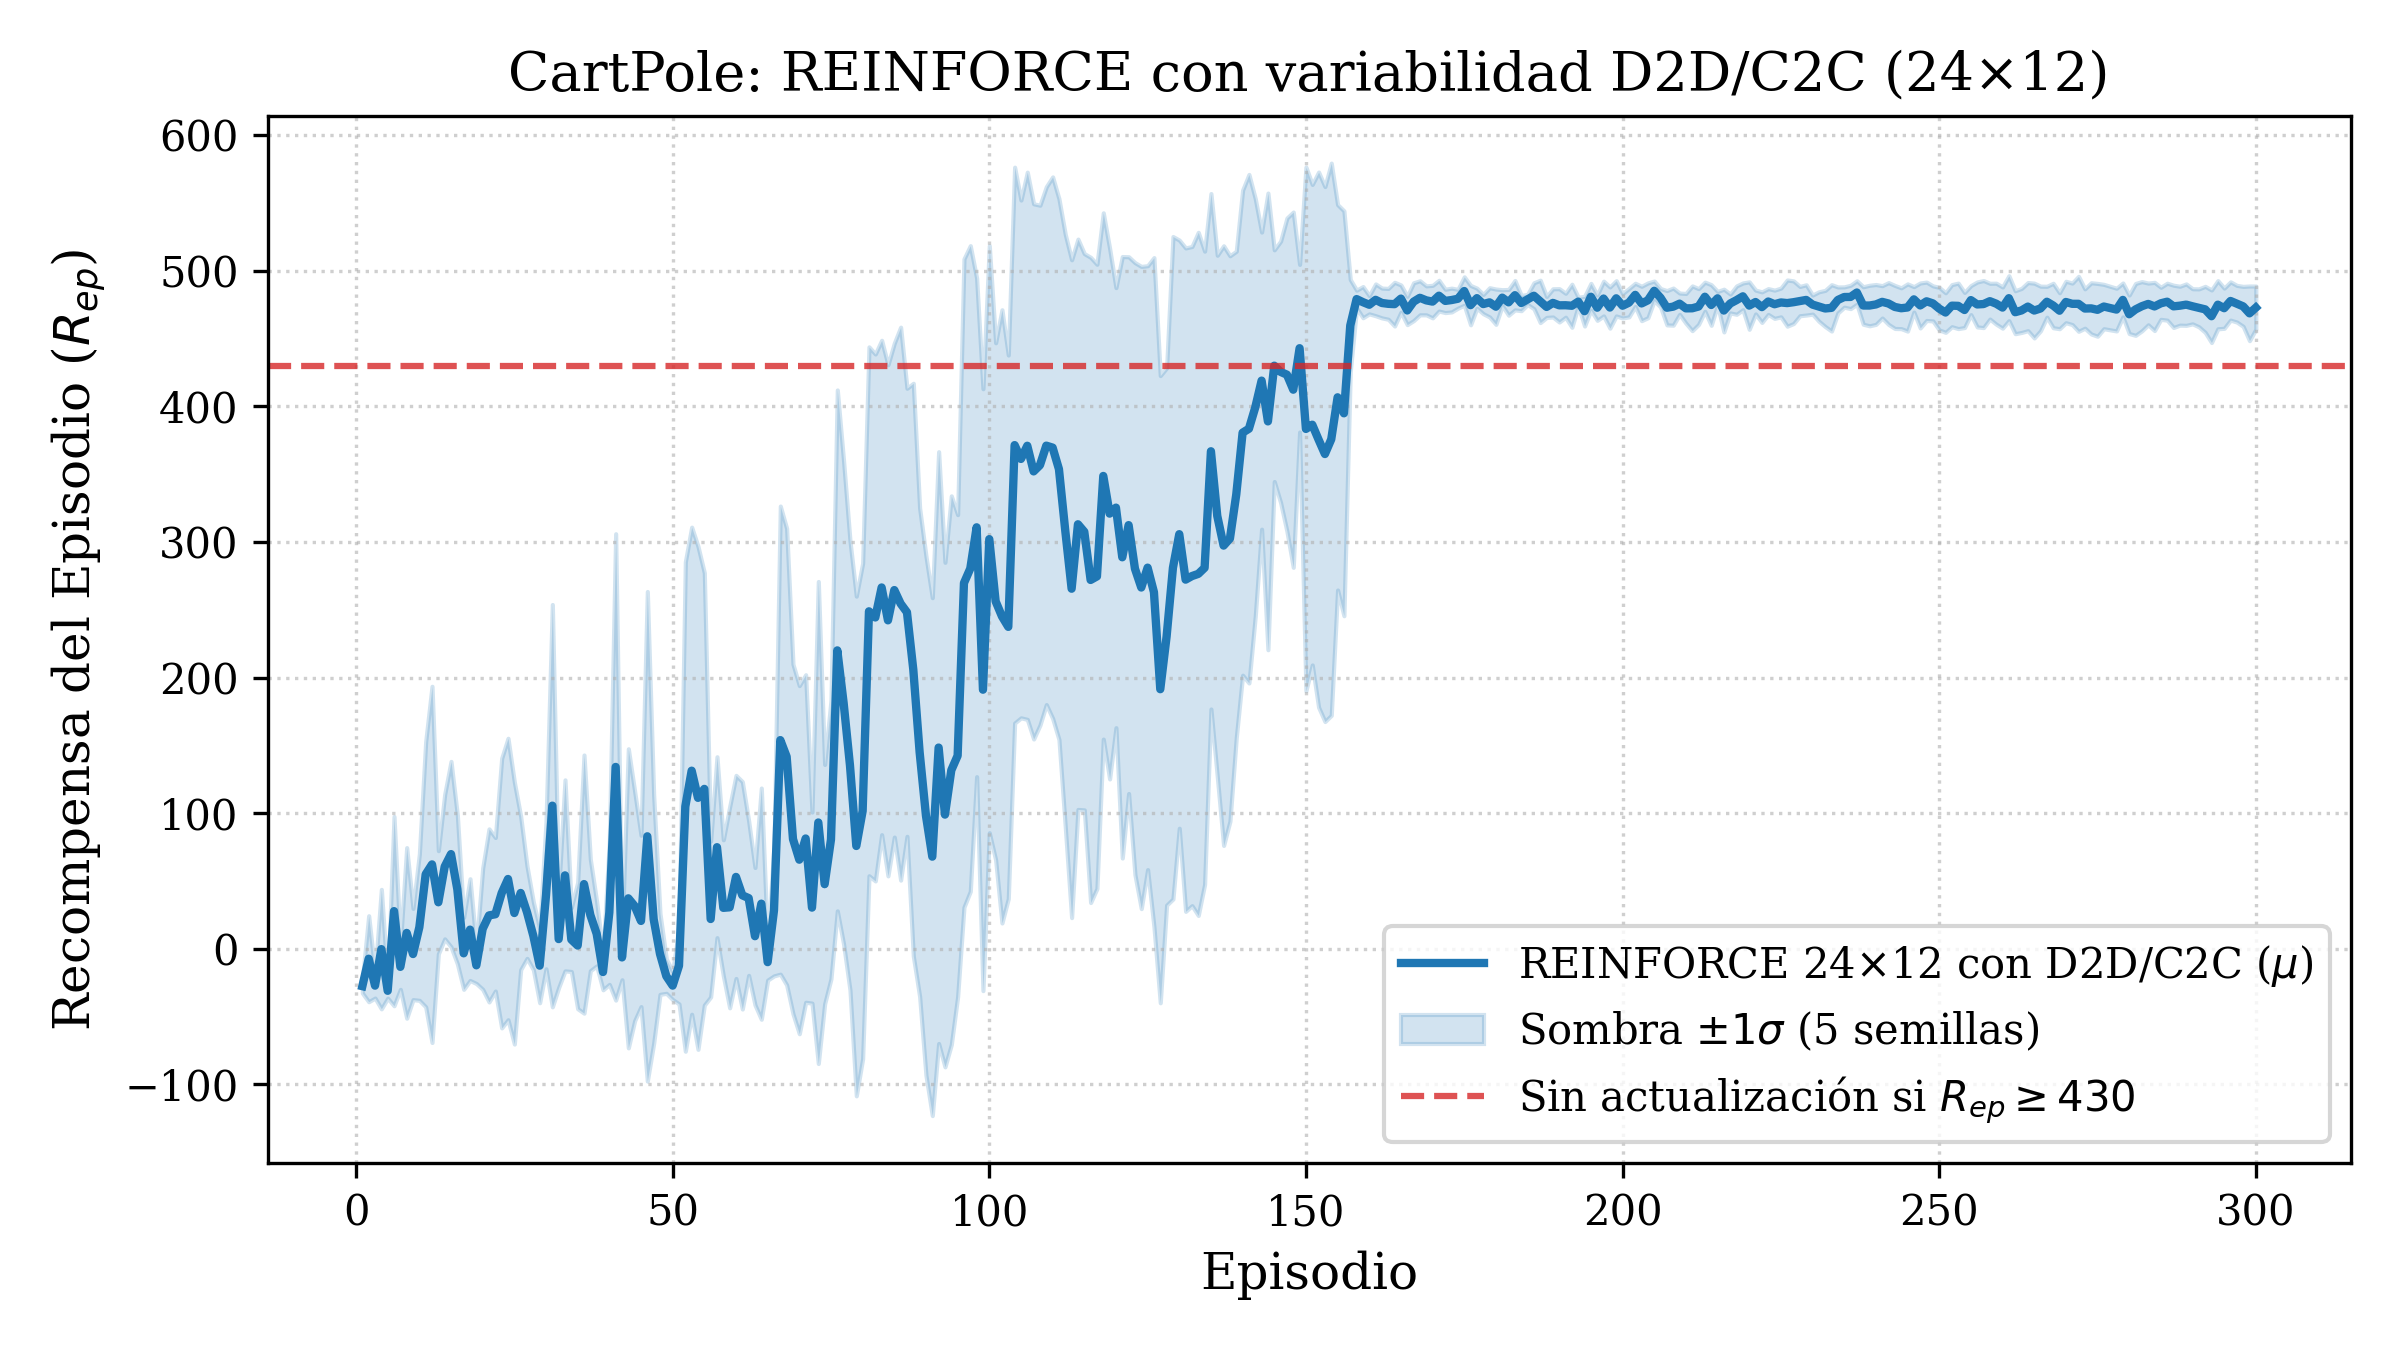
\includegraphics[width=0.76\textwidth]{figuras/cartpole_learning_24x12_5seeds_d2d_c2c.png}
\caption{Recompensa de cinco corridas CartPole con D2D/C2C, suavizada para facilitar la lectura.}
\label{fig:cartpole_learning}
\end{figure}

\subsection{Visi\'on $8\times8$: clasificaci\'on supervisada}
\label{sec:res_vision}

La tarea clasific\'o ocho patrones binarios mediante un crossbar $64\times8$.
En tres corridas de 5000 episodios, el acierto de los \'ultimos 200 episodios
fue 100\%. Ese dato corresponde a las ocho plantillas del entrenamiento.
Para medir robustez se reservaron variantes con inversi\'on de p\'ixeles; tras
selecci\'on por validaci\'on, la semilla 2 obtuvo 42.5\% sobre 400 variantes
de test, frente a 12.5\% aleatorio. El test mide ruido sint\'etico sobre las
plantillas, no clases ni im\'agenes externas.

\begin{figure}[H]
\centering
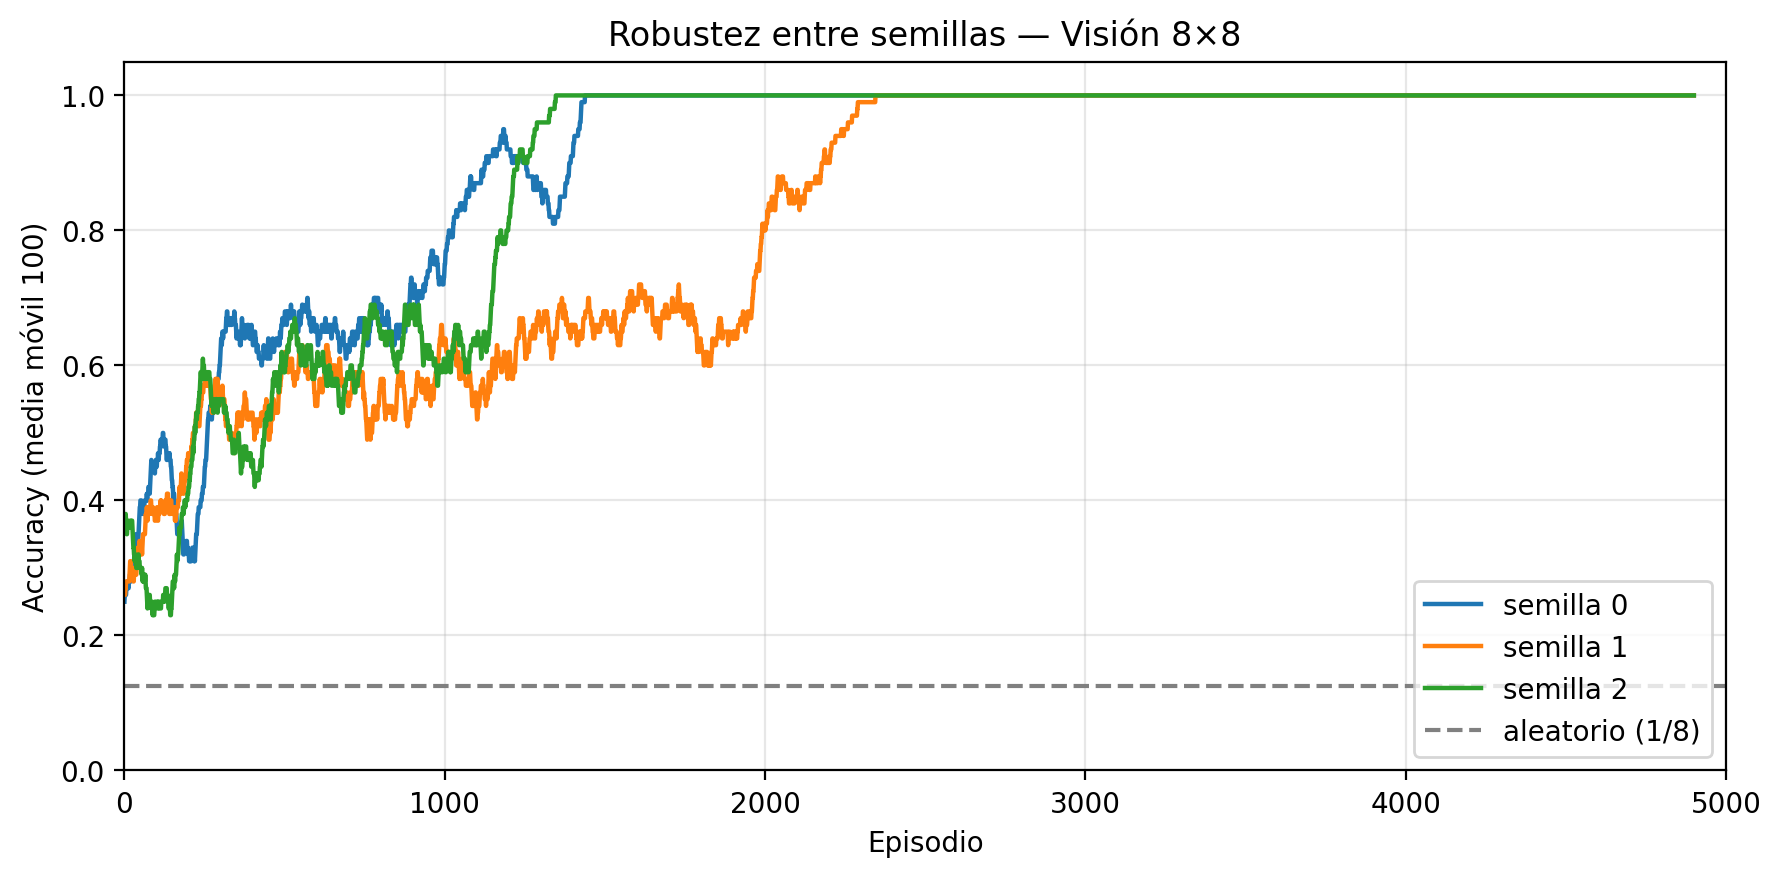
\includegraphics[width=0.72\textwidth]{figuras/vision_seeds.png}
\caption{Exactitud de tres corridas de visi\'on, suavizada con una ventana de 100 episodios.}
\label{fig:vision_seeds}
\end{figure}

\subsection{Navegaci\'on $10\times10$: control con recompensa escasa}
\label{sec:res_navegacion}

El gridworld contiene 15 obst\'aculos y cuatro movimientos, con recompensa
por llegar a la meta y penalizaciones por paso y colisi\'on. Las tasas de
\'exito de los \'ultimos 200 episodios fueron 100\%, 49.5\% y 82\% (media
no ponderada 77.17\%). En 50 mapas nuevos, el checkpoint seleccionado en
validaci\'on alcanz\'o la meta en 2 mapas (4\%). El buen resultado en el mapa
de entrenamiento no se transfiri\'o a mapas distintos en esta prueba. Los
registros de esa evaluaci\'on no est\'an incluidos como JSON recalculable y el
4\% se identifica como resultado reportado.

\begin{figure}[H]
\centering
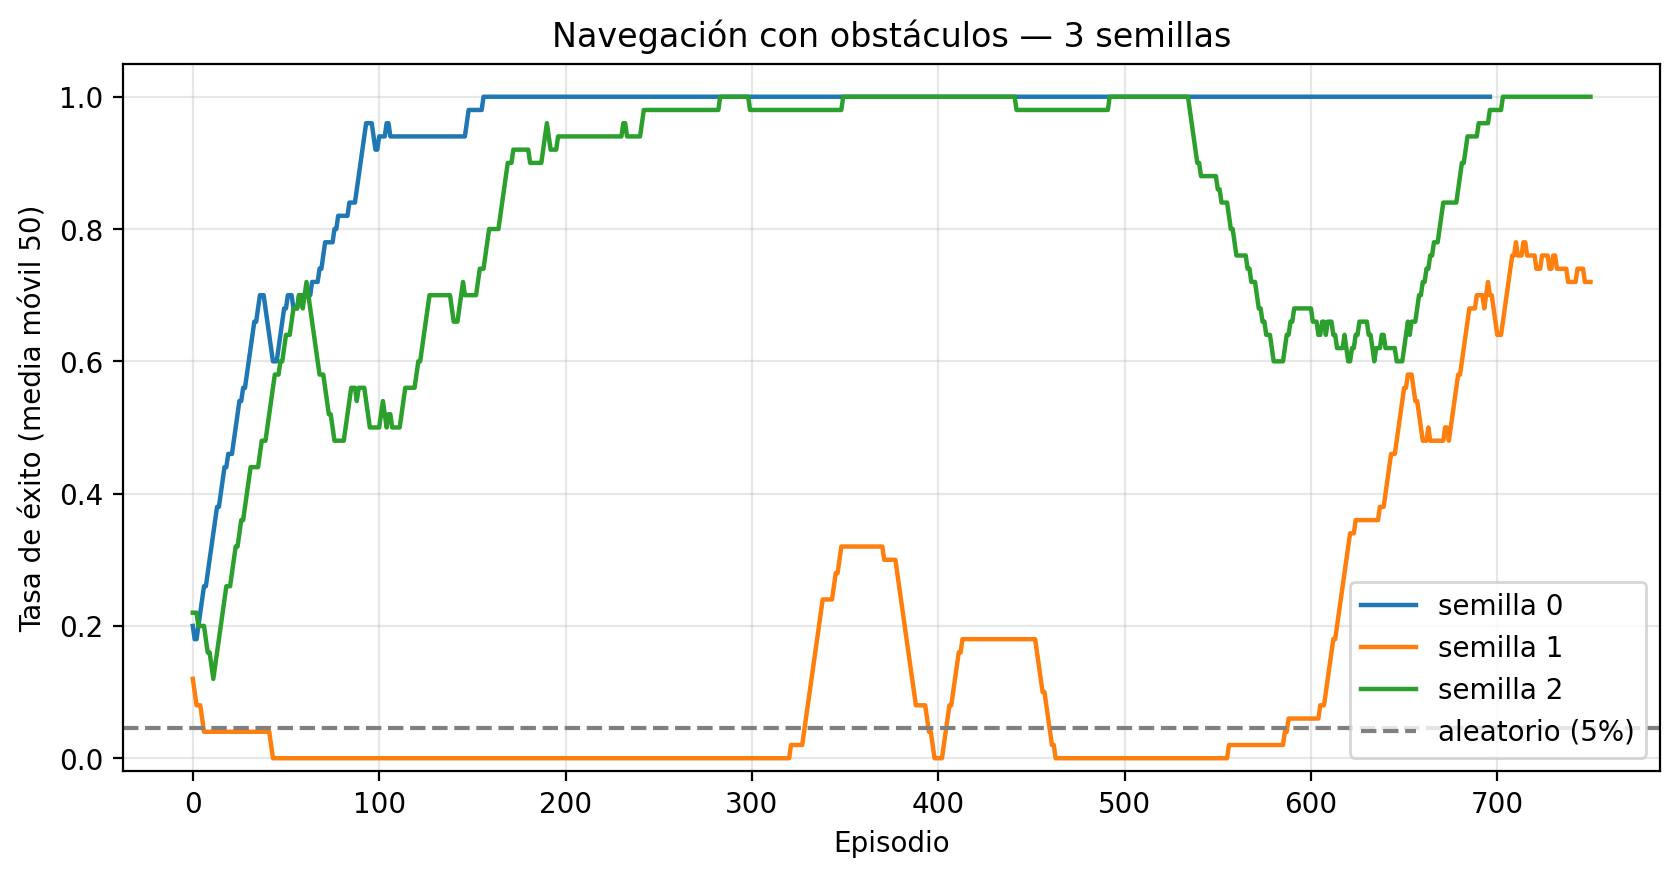
\includegraphics[width=0.72\textwidth]{figuras/obstacle_learning.png}
\caption{Tasa de \'exito de tres corridas del gridworld, suavizada con una ventana de 50 episodios.}
\label{fig:obstacle_learning}
\end{figure}

\subsection{Auto 2D: entorno continuo de conducci\'on}
\label{sec:res_auto2d}

El entorno combina ocho sensores de distancia, direcci\'on y cuatro controles,
con crossbar $24\times8$. El registro disponible indica 5.0\% de \'exito en
los \'ultimos 200 episodios; una evaluaci\'on reportada obtuvo 14\% (7/50) en
test. Solo existe una semilla y faltan los archivos necesarios para
reconstruir la curva y el checkpoint evaluado. Se considera un resultado
piloto, no evidencia de robustez entre semillas.

\subsection{An\'alisis comparativo entre tareas}
\label{sec:comparativa}
\label{sec:interpretacion_comparativa}

La Tabla~\ref{tab:cross_task} resume los \'ultimos 200 episodios de los
registros de presupuesto fijo. Recompensa, exactitud y tasa de llegada
son magnitudes diferentes; adem\'as, las tareas usan matrices y protocolos
distintos. La comparaci\'on es descriptiva y no estima un efecto causal de
la arquitectura ni de la regla de aprendizaje.

\begin{table}[H]
\centering
\small
\caption{Resumen descriptivo de las corridas de presupuesto fijo.}
\label{tab:cross_task}
\begin{tabular}{lccccc}
\toprule
Tarea & Episodios & Semillas & M\'etrica final & $\bar X$ & $\sigma_X$\\
\midrule
CartPole & 300 & 5 & $\bar R_{200}=435.31$ & 0.1379 & 0.0717\\
Visi\'on $8\times8$ & 5000 & 3 & $\mathrm{Acc}_{200}=100\%$ & $\approx0.10$ & 0.022--0.030\\
Navegaci\'on & 746--800 & 3 & $S_{200}=77.17\%$ & 0.221--0.345 & 0.190--0.288\\
Auto 2D & 1000 & 1 & $S_{200}=5.0\%$ & 0.319 & 0.274\\
\bottomrule
\end{tabular}
\end{table}

\subsection{Piloto comparativo REINFORCE/R-STDP}
\label{sec:piloto_rstdp_reinforce}

El lote de parada por \'exito evalu\'o CartPole, visi\'on y obst\'aculos con ambos
algoritmos, semillas 0 y 1 e inicializaciones $X_0=0.1$ y $X_0=0.9$.
Car se ejecut\'o solo con R-STDP. El criterio fue al menos 271 \'exitos dentro
de los \'ultimos 300 episodios (90.33\%), con m\'aximo de 10\,000 episodios;
no exige 300 \'exitos consecutivos. Cada tarea conserva su tama\~no de crossbar
y definici\'on de \'exito. La tabla resume los registros del piloto.

\begin{table}[H]
\centering
\footnotesize
\begin{tabularx}{\textwidth}{l l p{1.5cm} X}
\toprule
Tarea & Regla & Criterio & Episodios / alcance\\
\midrule
CartPole & REINFORCE & 2/4 & 349 y 1249; dos registros incompletos a 559 y 1132.\\
CartPole & R-STDP & 4/4 & 307--1199 episodios.\\
Visi\'on & REINFORCE & 4/4 & 586--1357 episodios.\\
Visi\'on & R-STDP & 4/4 & 470--2951 episodios.\\
Obst\'aculos & REINFORCE & 4/4 & 300 episodios en las cuatro condiciones.\\
Obst\'aculos & R-STDP & 4/4 & 300--336 episodios.\\
Car, lote principal & R-STDP & 1/4 & Una condici\'on a 3775; tres a 10\,000 sin criterio.\\
Car, repetici\'on corregida & R-STDP & 2/4 & Semilla 2: 750 y 1548; semilla 4: ambas a 10\,000 sin criterio.\\
\bottomrule
\end{tabularx}
\caption{Resultado del piloto de parada por \'exito. Cada fracci\'on corresponde a cuatro condiciones semilla--$X_0$, salvo donde se indica el alcance incompleto.}
\label{tab:piloto_rstdp_reinforce}
\end{table}

R-STDP designa el modo implementado en el runner: elegibilidad local
modulada por retorno. La regla STDP local del crossbar s\'i produce cambios;
el piloto muestra que su integraci\'on con la tarea todav\'ia es inestable entre
condiciones y dominios. No se extrapola a hardware. La discusi\'on del evento
post, el baseline y la estabilidad est\'a en el Ap\'endice~\ref{ap:desarrollo_extendido}.

\subsection{Limitaciones}
\label{sec:limitaciones}

Los resultados son de simulaci\'on y no se dispone de un prototipo f\'isico.
Las comparaciones con art\'iculos usan datos digitalizados, a veces con pocos
puntos o protocolos incompletos; las pruebas sint\'eticas no sustituyen
mediciones. Las aplicaciones no comparten una m\'etrica ni un protocolo
id\'enticos. Visi\'on se evalu\'o con variantes de plantillas, navegaci\'on mostr\'o
baja transferencia a mapas nuevos y Auto 2D cuenta con una semilla y
archivos incompletos. El piloto R-STDP alcanza el criterio en algunas
condiciones, pero no permite concluir robustez general. Estas limitaciones
acotan las afirmaciones del trabajo y motivan m\'as semillas, registros
\'integros y protocolos previamente fijados.

\section{An\'alisis de costos}
\label{sec:analisis_costos}

El costo es una estimaci\'on acad\'emica de reproducir simulaciones en una
computadora disponible; no es un registro de gastos ni de horas efectivas.
Se imputan 260 horas a Bs.~20/h y asignaciones de equipo y servicios. No se
incluyen computadora nueva ni hardware memristivo f\'isico.

\begin{table}[H]
\centering
\small
\caption{Estimaci\'on acad\'emica de trabajo e infraestructura.}
\label{tab:costo_total}
\begin{tabular}{lrr}
\toprule
Concepto & Base estimada & Importe\\
\midrule
An\'alisis y dise\~no & 30 h $\times$ Bs.~20/h & Bs.~600\\
Desarrollo e implementaci\'on & 160 h $\times$ Bs.~20/h & Bs.~3\,200\\
Pruebas y validaci\'on & 35 h $\times$ Bs.~20/h & Bs.~700\\
Documentaci\'on y tesis & 35 h $\times$ Bs.~20/h & Bs.~700\\
Trabajo total & 260 h $\times$ Bs.~20/h & Bs.~5\,200\\
Uso de equipo disponible & Estimaci\'on & Bs.~400\\
Electricidad e internet & Estimaci\'on conjunta & Bs.~200\\
\midrule
Total acad\'emico referencial & & Bs.~5\,800\\
\bottomrule
\end{tabular}
\end{table}

Se consolidaron las categor\'ias de costo en una tabla para evitar repetir
los mismos importes en varios res\'umenes. Las tarifas son supuestos de
planificaci\'on, no comprobantes ni consumos medidos.
